\RequirePackage[l2tabu,orthodox]{nag}

% TODO: decide if one-sided/two-sided
\documentclass[headsepline,footsepline,footinclude=false,fontsize=11pt,paper=a4,listof=totoc,bibliography=totoc,BCOR=12mm,DIV=12]{scrbook} % two-sided
% \documentclass[headsepline,footsepline,footinclude=false,oneside,fontsize=11pt,paper=a4,listof=totoc,bibliography=totoc]{scrbook} % one-sided

\PassOptionsToPackage{table,svgnames,dvipsnames}{xcolor}

\usepackage[utf8]{inputenc}
\usepackage[T1]{fontenc}
\usepackage[sc]{mathpazo}
\usepackage[american]{babel}
\usepackage[autostyle]{csquotes}
\usepackage[%
  backend=biber,
  url=false,
  style=alphabetic,
  maxnames=4,
  minnames=3,
  maxbibnames=99,
  firstinits,
  uniquename=init]{biblatex} % TODO: adapt bibliography style
\usepackage{graphicx}
\usepackage{scrhack} % necessary for listings package
\usepackage{listings}
\usepackage{lstautogobble}
\usepackage{tikz}
\usepackage{pgfplots}
\usepackage{pgfplotstable}
\usepackage{booktabs}
\usepackage[final]{microtype}
\usepackage{caption}
\usepackage[hidelinks]{hyperref} % hidelinks removes colored boxes around references and links
\usepackage[toc,nonumberlist,acronym]{glossaries} % TODO: remove if glossary not needed
\usepackage{soul}         % for highlighting todo TODO: remove this
\usepackage{siunitx}      % show meu symbol for (micro-middleware)
\usepackage{lscape}       % to set a page in landscape mode
\usepackage{courier}      % source code in courier font
\usepackage{enumitem}     % custom spacing for enumrate and itemize
\usepackage{url}          % urls in references
\usepackage{color}        % listings have backgrounds
\usepackage{geometry}     % reduce spacing in Appendix
\bibliography{bibliography/literature}

\setkomafont{disposition}{\normalfont\bfseries} % use serif font for headings
\linespread{1.2} % adjust line spread for mathpazo font

\setlist[enumerate]{itemsep=-3pt}
\setlist[itemize]{itemsep=-3pt}

% Settings for lstlistings
\definecolor{light-gray}{gray}{0.95}
\lstset{%
  basicstyle=\footnotesize\ttfamily,
  breaklines=true,
  numbers=left,
  numbersep=5pt,
  backgroundcolor=\color{light-gray}
}

% Basic information for cover & title page
\newcommand*{\getUniversity}{Technische Universität München}
\newcommand*{\getFaculty}{Fakultät für Informatik}
\newcommand*{\getTitle}{Convergence Mechanisms for a Smart Space App Store}
\newcommand*{\getTitleGer}{Konvergenzmechanismen für einen App-Store für Smartspaces}
\newcommand*{\getAuthor}{Bibek Shrestha}
\newcommand*{\getDoctype}{Master's Thesis}
\newcommand*{\getSupervisor}{Prof. Dr.-Ing. Georg Carle}
\newcommand*{\getAdvisor}{Marc-Oliver Pahl and Benjamin Hof}
\newcommand*{\getSubmissionDate}{17. November 2014}
\newcommand*{\getSubmissionLocation}{Munich}

% TODO: add custom commands etc.


% TODO: remove if glossary not needed
\newglossaryentry{computer}
{
  name=computer,
  description={is a machine that\ldots}
}

\newacronym{tum}{TUM}{Technische Universität München}


\begin{document}

\begin{titlepage}
  % HACK for two-sided documents: ignore binding correction for cover page.
  % Adapted from Markus Kohm's KOMA-Script titlepage=firstiscover handling.
  % See http://mirrors.ctan.org/macros/latex/contrib/koma-script/scrkernel-title.dtx,
  % \maketitle macro.
  \oddsidemargin=\evensidemargin\relax
  \textwidth=\dimexpr\paperwidth-2\evensidemargin-2in\relax
  \hsize=\textwidth\relax

  \centering

  \vspace{40mm}
  \includegraphics[width=40mm]{logos/tum}

  \vspace{5mm}
  {\huge\MakeUppercase{\getFaculty{}}}\\

  \vspace{5mm}
  {\large\MakeUppercase{\getUniversity{}}}\\

  \vspace{20mm}
  {\Large \getDoctype{}}

  \vspace{15mm}
  {\huge\bfseries \getTitle{}}

  \vspace{15mm}
  {\LARGE \getAuthor{}}

  \vspace{20mm}
  \includegraphics[width=20mm]{logos/faculty}
\end{titlepage}


\frontmatter{}

\begin{titlepage}
  \centering

  \vspace{40mm}
  \includegraphics[width=40mm]{logos/tum}

  \vspace{5mm}
  {\huge\MakeUppercase{\getFaculty{}}}\\

  \vspace{5mm}
  {\large\MakeUppercase{\getUniversity{}}}\\

  \vspace{20mm}
  {\Large \getDoctype{}}

  \vspace{15mm}
  {\huge\bfseries \getTitle{}}

  \vspace{10mm}
  {\huge\bfseries \getTitleGer{}}

  \vspace{15mm}
  \begin{tabular}{l l}
    Author: & \getAuthor{} \\
    Supervisor: & \getSupervisor{} \\
    Advisor: & \getAdvisor{} \\
    Submission Date: & \getSubmissionDate{} \\
  \end{tabular}

  \vspace{20mm}
  \includegraphics[width=20mm]{logos/faculty}
\end{titlepage}

\thispagestyle{empty}
\vspace*{0.8\textheight}
\noindent
I assure the single handed composition of this \MakeLowercase{\getDoctype{}} only supported by declared resources.

\vspace{15mm}
\noindent
\getSubmissionLocation{}, \getSubmissionDate{} \hspace{5cm} \getAuthor{}

\cleardoublepage{}

\addcontentsline{toc}{chapter}{Acknowledgments}
\thispagestyle{empty}

\vspace*{2cm}

\begin{center}
{\usekomafont{section} Acknowledgments}
\end{center}

\vspace{1cm}

I would like to thank my supervisor, Prof. Dr.-Ing. Georg Carle and my advisors Dr. Marc-Oliver Pahl and Mr. Benjamin Hof for the opportunity to work on this thesis, and their patience and constant guidance throughout the work.

\cleardoublepage{}

\chapter{\abstractname}

Smart Spaces are an exciting area with plenty of existing research. Different advanced have been made in smart devices, network standards and protocols and software systems. Still, there are challenges to build software systems that can run in multitude of different enviroments with variety of different smart devices. There are also challenges to write interoperable software systems.

A similar problem existed for softwares written for mobile devices. But in the last ten years, Apple has democratized the software distribution landscape by introducing the App Store. App store provides a central place of software distribution with equal reach to developers and users from anywhere in the world. Democratization of software development for Spart Spaces is waiting to happen and has been envisioned by S2Store, an app store for Smart Spaces. 

S2Store supports applications written on top of a framework for smart spaces known as ``Distributed Smart Space Orchestration System (DS2OS''. S2Store and DS2OS do not define any default standards for hardwares devices or default communication protocols etc. However the major challenge for S2Store is to engage developers and users such that their activities lead towards convergence and thus emergence of standards selected by the community.

The thesis presents different mechanisms suitable for S2Store to support the process of convergence. A simulation of S2Store with selected reputation systems called S2Eco is created. It is then used to study the evolution of the smart space ecosystem and to confirm that the reputation mechanisms lead to desired converngence.

\microtypesetup{protrusion=false}
\tableofcontents{}
\microtypesetup{protrusion=true}

\mainmatter{}

\chapter{Introduction}

\section{Background}

Mark Weiser in his landmark article ``The computer for the 21st century'' \cite{Weiser1991} explains Ubiquitous Computing as technology that disappears in the background and becomes invisible to the user. ``The most profound technologies are those that disappear'' \cite{Weiser1991}. \emph{Disappearing} means the forms in which they exist around us change. They blend into the background and get out of our way so we can just go about our lives. They would be present everywhere and their presence would improve the efficiency of doing our daily activities. Our everyday experiences with physical objects are enhanced because their forms are interconnected, aware and therefore intelligent.

After 13 years since Weiser published his paper, we have made significant progresses towards his vision. Internet has evolved from being just an interconnection of hyperlinked objects. It is now a global resource on top of which, complex infrastructures can be built. Sensors can be connected to harvest information from the environment, actuators can be used to interact with the environment. Services like data transformation, mining, analysis, storage, etc are readily available through the internet. Fuelled by availability of open wireless technologies like WiFi, RFID, Bluetooth as well as embedded sensors and actuators nodes, Ubiquitous Computing has stepped out of its infancy and in the verge of transforming current static Internet into a full fledged Future Internet \cite{Gubbi2013}.

Cook and Das says that this advancement has allowed researches and practitioners to create a wide variety of pervasive computing systems that reason intelligently, act autonomously, and respond to the needs of the users in a context and situation aware manner \cite{Cook2012}. On the one hand, the field has matured to the point where tangible, beneficial prototype testbeds such as smart homes, body area networks, health monitoring systems, and mobile social networking media are becoming fairly commonplace \cite{Cook2012}. These visible successes are built on mature underlying technology that performs smart device communications, resource discovery, information fusion, dissemination and routing, location tracking, activity recognition, and learning of user preferences. On the other hand, however, these systems have been mostly designed and tested on small to medium-scale applications with limited dissemination of the tools, results, and datasets \cite{Cook2012}.

When comparison to smartphone ecosystems, similar trend can be seen. Several companies introduced innovative technologies with their own operating systems like Symbian, Windows CE, MeeGo etc. They included features like camera, touch screen, QWERTY keyboards as well as apps to take notes, send emails, track reminders, browse internet etc. But there was no dominant platform until Apple introduced the iPhone in June 2007. The iPhone not only changed the user experience by removing the keypad and introducing a larger touch screen, it also offered a triangular relationship between third party developers, consumers and the iOS operating system by introducing Apple's App Store on July 10, 2008 \cite{wiki:AppStore_iOS}. App Store became a central market place. Users could buy quality apps from developers. This quickly gave rise to the iOS ecosystem that overtook existing ecosystems in terms of popularity and use.

The name \emph{App Store} is associated to Apple Inc's digital distribution platform for iOS applications. After its popularity and the launch of similar services by competitors, the term \emph{app store} has been adopted to refer to any similar service for mobile devices. We use the later common definition when we refer to app stores. 

App store is an integral part of the ecosystem of many different software platform. It comes in various forms. For programming language there exist software repositories like CPAN, PyPI, RubyGems, Maven, Boost, PEAR etc. For operating systems there are \textit{homebrew} for OSX, \textit{yum}, \textit{apt}, \textit{pacman} etc for linux distributions. Other platforms like github, sourceforge exist that hosts source codes of different projects. Similarly other mobile operating systems have application distribution channels: Like Apple's \emph{App Store} for iOS devices, Android devices use the \textit{Play Store}, Windows devices use \emph{Windows Phone Store} etc.

Ian Murdock when asked ``What single biggest advancement Linux has brought to the industry?'' replies ``Package management: or, more specifically, the ability to install and upgrade software over the network in a seamlessly integrated fashion along with the distributed development model package management enabled'' \cite{murdock_how_package_management}. \cite{Jansen} writes the benefits of app store as:

\begin{enumerate}
  \item For a developer, app store allows to publish her applications in one central place where people can find it.
  \item People become more aware of app business and app economy.
  \item An app store is the method of choice to build engaging and vibrant software ecosystems.
  \item an app store allows users to discover new apps in different categories and install them easily.
\end{enumerate}

This can be seen by observing the growth of different ecosystems. E.g. in mobile, the iOS and Android ecosystems had exponential growth in the last six years. Apple introduced \textit{App Store} in 2008 with an initial 500 native apps \cite{applefivehundrednatievapps}. It grew to 1.12 million apps in June, 2014 \cite{appstoretwelvemillionapps}. Similarly Android PlayStore has grown from 2300 apps in March, 2009 to 1.2 million in June, 2014 \cite{wpandroidhistory} as can be seen from Figure \ref{fig:app-bar-chart-3}.

\begin{figure}
  \centering
  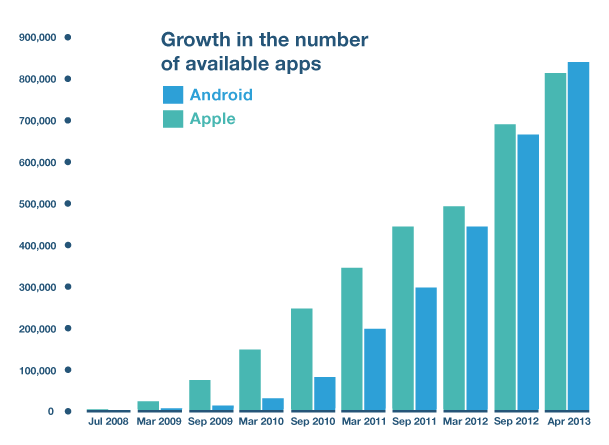
\includegraphics[width=13cm]{figures/app-bar-chart-3.png}
  \caption{Comparison of growth in number of available apps in App Store and Play Store. Source: http://www.appdomains.com/app-promotion/app-market-overview/}
  \label{fig:app-bar-chart-3}
\end{figure}

In the last four years, user contributed libraries for ruby programming language in http://rubygems.org have increased from 10,000 to more than 90,000 as the ruby language has gathered popularity \cite{modulecounts}. More recent examples would include Docker and Atom.io. Docker is an open-source project that automates the deployment of applications inside software containers. To promote more developer engagement, docker introduced Docker hub \cite{dockerhub}\cite{wiki:Docker_Software} where people can openly share their docker images. Similarly Atom.io calls themselves ``A hackable text editor for the 21st Century''. It also contains a repository for developers to contribute packages and themes \cite{atomiorepo}\cite{wiki:Atom_TextEditor}. Package contributions for both softwares have increased in the past few months.

The benefits of an app store can apply equally to Ubiquitous Computing platforms. \cite{dixon2010home} describe HomeOS and HomeStore. HomeOS is an operating system for managing different smart devices to create smart environment inside a home. Software developers can build applications and share them online in HomeStore, which is an app store for HomeOS similar to Apple's App Store for iOS. HomeStore recommends users with different software they can run inside their house. It also recommends the user about missing smart devices necessary to run certain applications. HomeStore also performs basic quality checks and supports ratings and reviews to help identify harmful or badly engineered applications.

Pahl recently completed his Ph.D. thesis on \emph{Distributed Smart Space Orchestration System (DS2OS)} \cite{pahl2014distributed}. He describes DS2OS as a platform that allows orchestration of smart environments. It includes a Software Development Kit (SDK) for developers to create different types of applications for smart spaces. It provides a runtime environment to run the software in distributed environment. DS2OS also consists of an app store named S2Store. Like with HomeStore for HomeOS and App Store for iOS, S2Store is a marketplace for smart space applications.

\section{Objective}

\cite{pahl2014distributed} list the two major challenges in Ubiquitous Computing platform which an app store can help overcome and explains how. The challenges being:

\begin{enumerate}
  \item Smart spaces have huge diversity of smart devices.
  \item Smart spaces have diversity of orchestration scenarios.
\end{enumerate}

\emph{Diversity of smart devices} means the existince of a wide variety of devices in the market available from different vendors. For mobile devices, the available hardwares are bound to predefined specifications. Most mobile devices have standard sensors and standard hardware parts. Applications build for mobile devices have less incompatibility issues. In contrast, electronic hardwares have no widely accepted standards when it comes to features. For e.g., a table lamp could vary in working from another table lamp from different vendor in the brightness of the bulb, the size of the lamp, lamp made for wall versus for the table, if it allows dimming the lamp, etc. Integration of these devices into pervasive computing environments require special hardware drivers. It is unlikely that vendors provide hardwares drivers for their devices when there isn't any standard platform.

\emph{Diversity of orchestration scenarios} means that there exists many different ways to orchestrate a smart space. For e.g., it is highly like for two houses to have different room structure, different requirements for entertainment, different interest of the house owners, etc. The kinds of different applications that can be written for all the different scenarios are huge. It is desired that applications are written in small and modular fashion and can interoperate with each other. Larger complex functionality is achieved by reusing smaller modules together. Such system does not exist for smart spaces.

The DS2OS framework with S2Store solves these issues by allowing crowdsourced development. Crowdsourcing is the process of obtaining needed services, ideas, or content by soliciting contributions from a large group of people \cite{pahl2014distributed}. Crowdsourced software development means software developers contributing to S2Store on a global scale. In S2Store, there are different entities that can be contributed by the crowd as described in Section \ref{sec:ds2os}.

Crowdsourcing results in:

\begin{enumerate}
  \item Large number of contributions and
  \item Varying quality of contributions.
\end{enumerate}

It is desirable to have large number of contributions in online app store. But, varying quality of contributions caused by varying skill, knowledge and experience of developers has to be taken into consideration. Identification of quality contents in large crowdsourced platforms is a common problem. Online marketplaces e.g. eBay, Amazon, StackOverflow uses reputation systems that label whether a certain user or the item she wants to trade, is good or bad, trustworthy or fake. Reputation Systems are special features added to online marketplace to create trust among users and mark qualities of different items. \cite{Resnick2000} and \cite{farmer2010building} describe reputation systems in detail.

An app store for smart spaces has similar requirements to that of any existing app stores for mobile platforms for trading purposes. In addition, an app store for smart spaces needs to consolidate challenge of having diverse hardware devices and orchestration scenarios. A smart space app store does this by creating a platform that allows collaboration of developers and early adopters to create standards themselves in a crowdsourced manner.

It is believed that given the vastness of the challenge present in developing softwares for smart spaces, reputation mechanisms are key parts of the solutions. The objective of the thesis is to understand the role of different reputation mechanisms in an online app store for smart spaces and how they play significant part by converging user opinions into default standards.
\chapter{Analysis}
\label{chap:analysis}

% \section{Smart spaces and middlewares}
\label{sec:smart_spaces}

Smart spaces are environments made up of different appliances that inter-work with each other and coordinate to proactively support the individuals in the environment for his/her daily activities. Smart spaces can refer to apartments, offices, museums, hospitals, schools, malls, university campuses and outdoor areas that are enabled for co-operation of smart objects and systems.

Mark Weiser envisioned smart spaces in 1991 as omnipresent computing devices spread out in the envirornmnet such that for humans their computing nature is oblivious \cite{Weiser1991}. He presented three technical requirements for the realization of smart spaces \cite{Weiser1991}\cite{pahl2014distributed}:

\begin{itemize}
  \item ``cheap, low-power computers that include equally convenient displays,''
  \item ``software for ubiquitous applications, and''
  \item ``a network that ties everything together''.
\end{itemize}

The vision of computers that interact with people's regular environments (``everyday's fabric'') is not reality in 2014 \cite{pahl2014distributed}. We present a short discussion on state of art by dividing the requirements under three items.

\subsection*{a. Devices}

Most smart devices are those that have wired or wireless network interfaces. Often used devices for household or office purposes are already available in the ``smart'' variants. Traditional non-smart devices have one specific purpose: fulfill the purpose of their utility in isolation. The newer appliances go beyond this by integrating extra computing units and network interfaces so they can be connected to a network. Smart devices in the professional and consumer domains are available and growing in their number 2014 \cite{pahl2014distributed}.

\begin{figure}
  \centering
  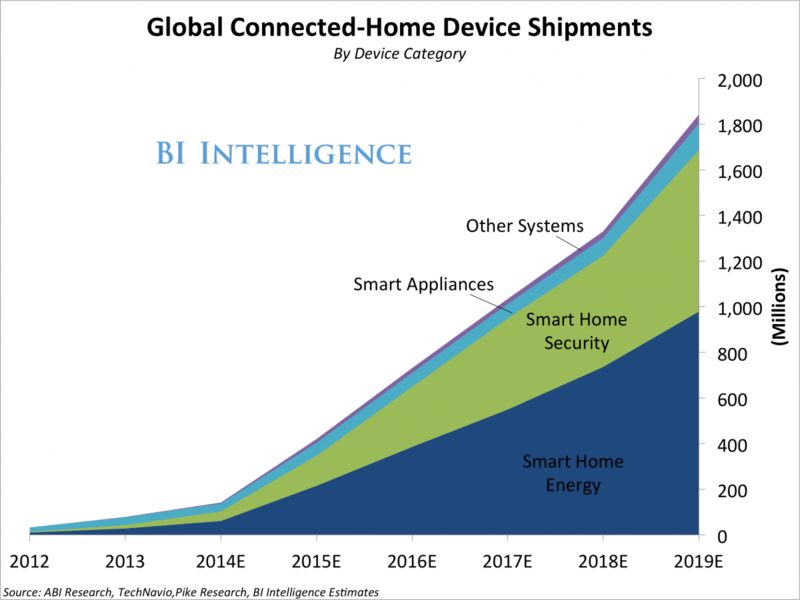
\includegraphics[width=10cm]{figures/connectedhomedevicecategories-1.png}
  \caption{Growth prediction of global connected home device shipments.}
  \label{fig:growth_home_device_with_categories}
\end{figure}

\subsection*{b. Networks}

In 2014, advancements in wired and wireless technologies have been achieved that allow sufficient bandwidth across short and long distance communications. WiFi technology is widely accepted to create networks in smaller spaces. Cellular networks provide highspeed connection to the Internet with third generation (3G) and fourth generation (4G) Long-Term Evolution (LTE) networks. Wireless networking standards like ZigBee, NFC, RFID and Bluetooth are used by small low powered digital radios \cite{warriach2013state}. Connectivity on physical level is already achieved. The challenge is to connect different types of devices (heterogeneous devices) on a semantic level \cite{pahl2014distributed}.

\subsection*{c. Softwares}

There already exists softwares that allow distributed computing. Technology like cloud-computing allows tasks to be divided and run in multiple computers. Software as a service (SAAS) providers have developed browser based applications for real time online collaboration across different types of devices. A part of the original vision has been achieved because we as humans have more advanced ways of collaborating with each other through computers. But computers have not disappeared into the background yet.

Softwares for pervasive computing have been a topic of wide research. These researches have focussed in different domains like health care and well being, e-Learning and campus life, tourism and traveling, office and other business applications, security and safety, energy saving, advertising and e-commerce, entertainment, user convenience, gaming, and social community applications \cite{pahl2014distributed}. When smart devices are managed via a software to create a smart space, it is called \emph{software orchestration}. Typically, the research projects implement software and hardware in exactly the same circumstances as the ones used during the research. The softwares that are produced are limited to their own domain and the domain environment, unsuitable for a different domain.

Marc-Oliver Pahl in his PhD dissertation described a new system called ``Distributed Smart Space Orchestration System (DS2OS)'' that presents a better approach of software orchestration \cite{pahl2014distributed}. DS2OS provides an open and portable middleware softare that can be used as a framework to develop new pervasive computing applications for wide variety of pervasive computing scenarios. DS2OS and its features are further described in Section \ref{sec:ds2os}.

\subsection*{Conclusion}

For all three requirements: devices, software and network already exists for pervasive computing scenario. The challenge is to build a platform that easily scales to the requirements of different domains and yet provides interoperability between them.

Further detailed state of the art for smart space middlewares and the networking technologies have been discussed in \cite{warriach2013state} and \cite{pahl2014distributed}.
% \section{Device Heterogeneity}
\label{sec:device_heterogeneity_and_portability}

\emph{Device Heterogeneity} means the availability of different varieties of devices on the market. Different hardwares have different interfaces that connect the real world with the digital world. The amount of heterogeneity in hardwares can be understood by studying their classification into two use domains.

\begin{itemize}
  \item Professional building automation domain,
  \item Home automation domain.
\end{itemize}

\subsection*{Professional building automation domain}

This domain includes hardware devices used in large industrial scale buildings to orchestrate, mechanize and aggregate data of smart devices \cite{pahl2014distributed}. The systems used are called Building Automation Systems (BASs). Smart Devices build for BAS have typically standardized interfaces. Due to this, softwares are portable with devices from multiple vendors. The number of companies that dominate the market is small. Which makes standardization possible. Some BAS controllers also provide a vendor independent management interface to remote control devices from outside e.g. Open Building Information Exchange (oBIX) and BACnet. However BAC systems are complex and expensive for home users.

\subsection*{Home automation domain}

Home automation is done on a smaller scale. Home users have wider variety of devices available from a lot of independent vendors. The devices are cheaper than BACs hardwares. Home automation typically use medium and low priced vendor proprietary solutions for domains such as heating, lighting, safety and security, comfort, energy management, remote management, etc.

Smart devices for home automation also vary in the type of communication protocols. For e.g., X10 over Power Line Communication (PLC), CEBus over different media, LonWorks, KNX, Ethernet, X801.11, etc are some of the popular communication protocols \cite{warriach2013state}. It is also usual for vendors to lock-in the users by not publishing the specifications to their hardware interfaces or providing only proprietary device drivers. Thus the amount of standardization among different vendors is low.

The assessment is that where there is standardization, there exist limited vendors that supply expensive hardwares only affordable on BACs. For general users, the affordable devices lack standardization.

\subsection{Overcome heterogeneity}

Standardization is a primary requirement for interoperable softwares. Different strategies to bring standardization and overcome heterogeneity is analysed in \cite{pahl2014distributed} by \emph{Heterogeneity Bridging}. In Heterogeneity Bridging, the architecture for software orchestration is broken down into three different functional layers:

\begin{itemize}
  \item In the orchestration services.
  \item ``In the middle'' explained further in Section \ref{sec:ds2os}.
  \item On the Smart devices.
\end{itemize}

\cite{pahl2014distributed} argues that the best layer for \emph{Heterogeneity Bridging} is the \emph{middle layer}. 

The \emph{middle layer} decouples the dependency between the layer of physical hardware devices and the layer of software devices by providing the concept of hardware interface abstraction. The communication between an application and a smart device is done through abstract interfaces of the device. The abstract interfaces are vendor independent. Both orchestration services and the smart devices remain simple by avoiding coupling logic. Multiple services can use the same abstract interface to communicate with a smart device.

\subsection*{Conclusion}

The introduction of \emph{middle layer} and hardware interface abstraction is a viable solution to device heterogeneity.
\section{Distributed Smart Space Orchestration System}
\label{sec:ds2os}

Distributed Smart Space Orchestration System (DS2OS) is a framework that allows orchestration of a collection of smart devices together to create different types of intelligent smart environments \cite{pahl2014distributed}. 

DS2OS consists of three main building blocks:

\begin{enumerate}
  \item The Virtual State Layer (VSL) \si{\micro}-middleware (Middle Layer).
  \item The Service-to-Space (S2S) service management framework.
  \item The Smart Space Store (S2Store).
\end{enumerate}

\textbf{The Virtual State Layer (VSL) \si{\micro}-middleware} is introduced in \cite{pahl2013missing}\cite{pahl2014distributed}. Virtual State Layer (VSL) is a representation that allows abstraction of smart devices and their orchestration to form smart spaces. VSL virtualizes the real world of sensors and actuators in a software environment called ``middleware''. A middleware then facilitates creation of softwares that can easily use these abstract representations to create advanced smart spaces.

Traditionally middlewares are domain specific: they cater to domain specific devices and domain specific orchestration scenarios. Pahl calls the domain specific middlewares as \emph{silos}. These silos lack interoperability and reuse. E.g., an intrusion detection system for a large warehouse and similar system for home automation are likely to use different middleware systems although they share similar requirements.

VSL as a \si{\micro}-middleware differs from other smart space middlewares because it is not limited to any specific domain.

VSL requires that hardware devices are abstracted into meta devices called \emph{context models} based on their utility. Hardware devices with similar features but different vendors can share the same context model. Hardware devices are linked with their respective context models in VSL by device specific software called gateway services.

VSL then provides features that allow any software system to communicate with the context models, thus decoupling a software system from the hardware device.

\textbf{The Service-to-Space (S2S) service management framework} provides a set of functionalities related to service management like service installation, uninstallation, starting, pausing, stopping and monitoring running services. Analogous to a mobile operating system that provides the necessary conditions to run mobile apps, the service management framework can run services developed for DS2OS. S2S handles services running in an environment consisting of distributed computing hosts.

\textbf{The Smart Space Store (S2Store)} is a web-based app Store that contains repositories for context models, access groups and services. It is a market for users to download applications suitable for their smart spaces. Users can provide feedback and/or rate applications. Developers can search and download existing context models and access groups and reuse them. User feedbacks as well as usage statistics of existing entities are used to calculate repuation for these entities.

The reputations are the central part of this thesis as we see the importance of their roles in Section \ref{sec:s2store_ecosystem}.

\begin{landscape}

  \begin{figure}
    \centering
    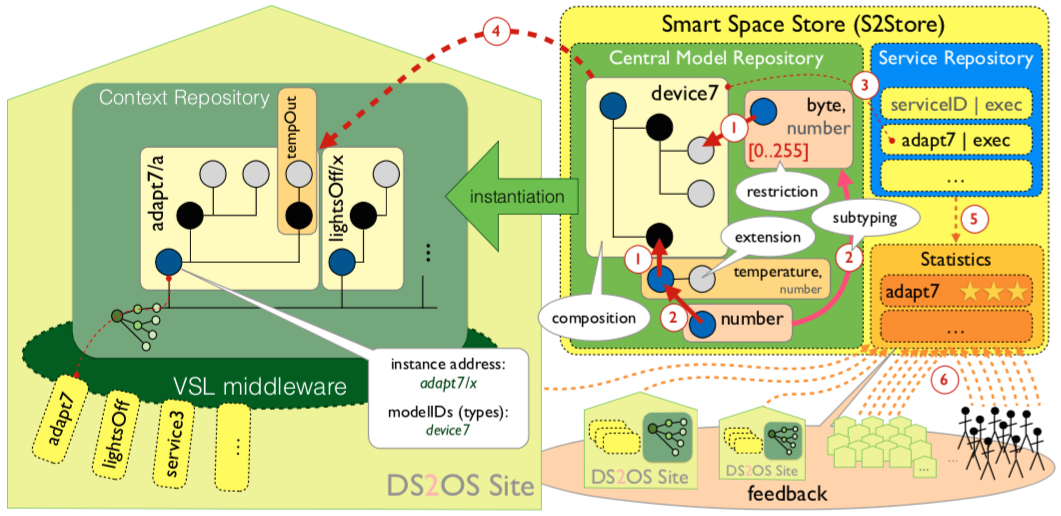
\includegraphics[width=21cm]{figures/ds2os.png} 
    \caption{Overview of DS2OS. (Source~\cite{pahl2014distributed})}
    \label{fig:ds2os}
  \end{figure}

\end{landscape}

\section{Portability and Support for Collaborative Convergence}
\label{sec:portability}

DS2OS architecture by design allows portability of software services and smart device.

Services are written in Java and packaged in standard Java Archive (jar) format. Services are portable because they run in all the platforms where Java Runtime is available given that the required smart devices are available in the platform. 

Services are also portable in the sense that they are not tied to a specific type and model of a smart device. Instead a service is compatible with a range of smart devices that share a common abstract interface (Context Models) in the VSL. Communication between the VSL context model and the device is done with adaptation services.

The result of portability of software services and smart device abstraction means they can be shared easily among other developers and users. Sharing is done by publishing them in the S2Store.

Portability causes sharability and sharability causes popularity. Popularity of services and context models reduces duplication. This process is called convergence.

Due to convergence, it is expected that there exists one popular context model among many that is compatible with as many similar diverse devices as possible. The side effect of convergence causes future smart device manufacturers to make sure that their devices are also compatible. Eventually convergence leads to automatic standardization.

The whole process is driven through the open platform provided by S2Store. And every individual developer has a equal hand in the process.

\subsection*{Conclusion}

DS2OS architecture provides portability of software services and context models. Portability combined with uploading in S2Store makes collaborative convergence and automatic standardization.


\section{Introduction to an app store}
\label{sec:introduction_to_an_app_store}

A software platform is comprised of the technology that makes up the platform as well as the human beings that use the technology. Over time, a platform has to evolve, under go changes, support more developers and reach out to more users of the platform. Most software platforms use app stores to support the growth process. \cite{Jansen} describes an app store as ``An online curated market-place that allows developers to sell and distribute their products to actors within one or more multi-sided software platform ecosystems.''

He describes that an app store system as one that should:

\begin{enumerate}
  \item be available using the internet,
  \item be curated by an organization, typically but not necessarily the platform owner,
  \item allow for the selling and buying of software products,
  \item take care of the financial transactions involved in selling the software products,
  \item have two distinct user groups: \emph{developers} and \emph{users},
  \item be serving one or more software ecosystem, and
  \item implement a platform that takes care of the distribution of the software products.
\end{enumerate}

\begin{figure}
  \centering
  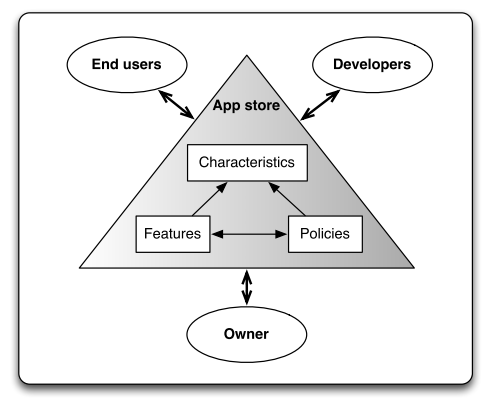
\includegraphics[width=9cm]{figures/app_store_triangle.png}
  \caption{Conceptual Model of an app store. (Source~\cite{Jansen})}
  \label{fig:conceptual_model_of_app_store}
\end{figure}

According to \cite{Jansen}, to create a better understanding of app store within the software ecosystem, a conceptual model is created as shown in Figure \ref{fig:conceptual_model_of_app_store}. The ovals show the actors involved in the ecosystem. The first one in the bottom is the owner of the app store. The second oval represents users, those who download and uses the apps. The third oval represents the developers who contributes and places their applications on the repository. They all interact with the triangle. The triangle represents the app store. The rectangles inside the triangle describe the processes inside the app store. The first rectangle represents Policies which act as guidelines for users and developers. The second rectangle represent Features. Both policies and features can be influenced by platform owner. The third rectangle represents the characteristics which cannot be directly influenced by the platform owner like the number of developers, number of users, quality of apps or the usability of the app store. However an owner can modify the policies and the features to influence the characteristics of the app store.

Features and policies complement each other. Features make an app store have more interesting ways for users to interact with. At the same time, the guidelines defined by Policies prevent the app store from being misused. Enforcing Policies are even harder than defining them. Big companies like Google and Apple have plenty of technical and human resources to check the quality of apps in their app stores. In smaller ecosystems, these resources are not readily available. Non the less, certain features can be introduced that makes enforcing policies easier. \cite{Jansen} studied six different mobile app stores: Google's PlayStore, Apple's App Store, SlideMe, Binpress, Amazon app store and Intel AppUp. They listed 69 characteristic features of a typical app store under 12 different categories. We list 6 features below that play part in convergence process.

\begin{itemize}
  \item \textbf{Recommendations} offer users new software based on their existing profile.
  \item \textbf{App categories} segregate Apps into distinct groups based on their features.
  \item \textbf{App lists} (e.g. top lists, latest additions) allow users to discover popular and new softwares.
  \item \textbf{Search} allow users to find the software by using plain text words.
  \item \textbf{Ratings} provide a feedback mechanism to other users know about the quality of software.
  \item \textbf{Review} are text comments describing users opinion of the software.
\end{itemize}

\section*{Conclusion}

App stores play a central role in a software platform. S2Store is the app store for pervasive computing platform DS2OS. It consists of features that allow developers to share context models and services. S2Store allows users to find and use uploaded services and provide feedback about their quality using S2Store's features. The analysis done in \cite{Jansen} is a good reference point for S2Store's feature sets.


\section{Reputation Systems}
\label{sec:reputation_systems}

On the internet, we interact with a lot of strangers. People can be anonymous. It is common to see individuals identify themselves only with a nick names \cite{Resnick2000}. In these circumstances, it is hard to build trust with each other. Online trade on the internet can be compared to the market of lemons as described in \cite{Akerlof1970}. A mechanism is required that incentivises individuals to act with honest intention. Internet scale systems use \textit{Reputation Systems} to foster trust between the users. A Reputation System collects, distributes and aggregates feedback about participants' past behaviours. Reputation systems require at least three properties \cite{Resnick2000}:

\begin{enumerate}
  \item Long-lived entities that inspire an expectation of future interaction;
  \item Capture and distribution of feedback about current interactions (such information must be visible in the future); and
  \item Use of feedback to guide trust decisions.
\end{enumerate}

Through reputation system, these properties can be applied to a) Users and b) Entities

\subsection{Reputation System for users}

Reputation system for users helps other individuals know what quality items to expect from a given user. Online systems like eBay, Amazon and other platforms that allow two sided transactions employ these techniques. On eBay, after a transaction is done, a buyer can leave either a positive, neutral or negative feedback for a seller. The feedback amounts to +1, 0 or -1 feedback points. A seller over a period of time accumulates feedback points from various buyers which becomes her feedback profile. A new buyer can use the feedback profile to decide if the seller is reliable enough.

\begin{figure}[!htb]
  \centering
  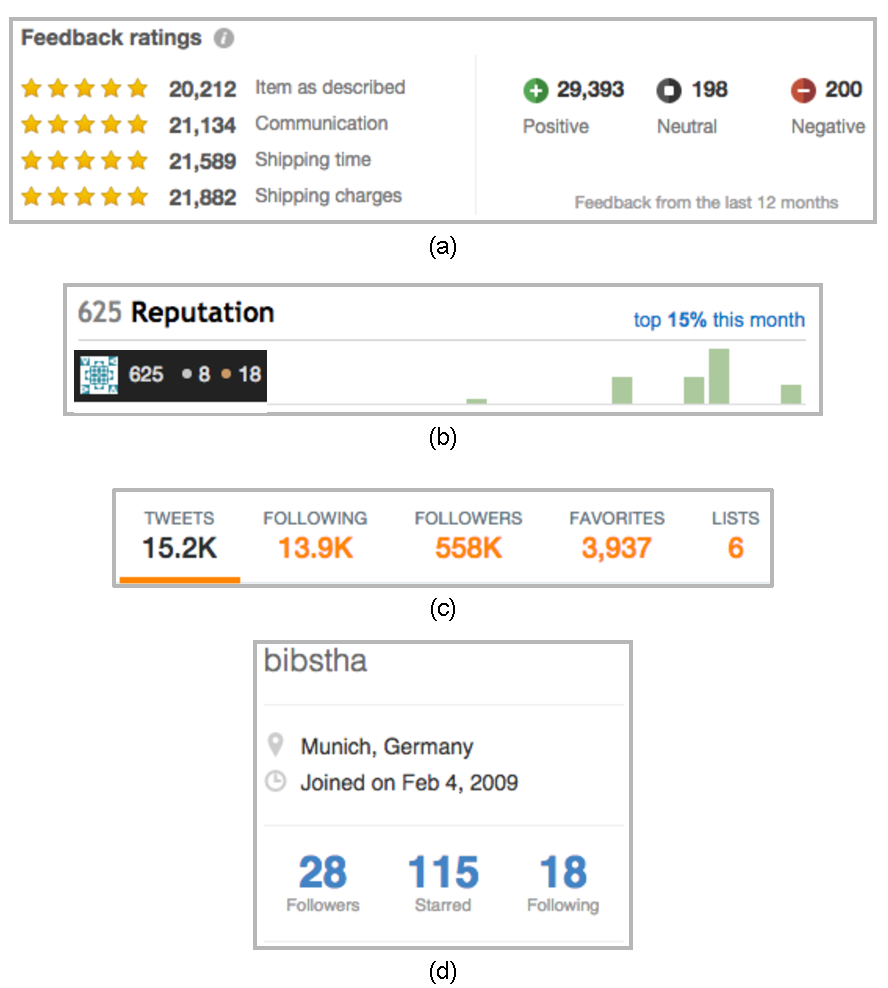
\includegraphics[width=11cm]{figures/rs_for_users.pdf} 
  \caption{Different reputation systems for users: (a) eBay feedback ratings, (b) StackOverflow User reputation, (c) Twitter reputation and (d) Github user follow information}
  \label{fig:rs_for_users}
\end{figure}

Reputation system for users also span beyond auction and e-commerce systems. QnA site  StackOverflow.com rates users by letting others choose the most helpful answers to a question. Users are encouraged to answer in the most comprehensive and helpful manner. This leads to higher quality answers. Product review sites (such as www.epinions.com) offer rating services for product reviewers (the better the review, the more points the reviewer receives).

Sites with \textit{follow} feature allow users to subscribe to the activities of other users. These systems build a directed graph structure. Each node is a user. Incoming vertices show people following the user while outgoing vertices show who she is following. Reputation is considered higher if she has high number of followers. In twitter.com, higher reputation means more people listen or like the users' posts. In github.com, higher reputation means more people are interested in the users' code contributions.

Reputation system for users portray a characteristic of a user. Political scientist Robert Axelrod calls this the ``Shadow of the future'' \cite{Axelrod1984}. An expectation that people will consider one another's pasts in future interactions constrains behaviour in the present.

\subsection{Reputation Systems for entities}

When trading on the Internet, it is not possible to directly interact with the items of trade. It is hard to determine the quality of products when there are multiple vendors selling products that are similar in visuals and written specifications. Reputation Systems for entities add visual measures as quality attributes. They gathers opinion from previous consumers to form a qualitative opinion of the entities and help new consumers form opinions.

\begin{figure}[!htb]
  \centering
  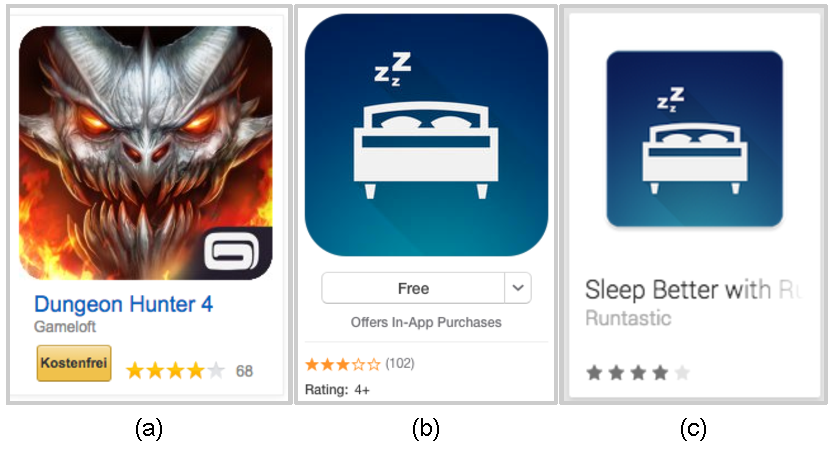
\includegraphics[width=12cm]{figures/rs_for_entities.pdf} 
  \caption{Different reputation systems for entities: (a) Amazon Appstore ratings, (b) Apple's Appstore ratings and (c) Google's PlayStore ratings}
  \label{fig:rs_for_entities}
\end{figure}

Reputation system for entities are used widely online. Amazon allows rating a product on a scale from 1 to 5 (1 very bad, 5 very good). Products of lower rating are assumed to be of lower quality and therefore make lower sales.

Apple's App Store and Google's Play Store only support reputation systems for entities. Both use the same model: users can rate an application in the scale of 1 to 5 stars (more stars means higher quality). App stores display the aggregate average. Apple's App store features categorization of ratings and reviews based on \emph{application versions}. This allows users to get more accurate review of the application based on current status. A developer can fix or update their applications based on user feedbacks. The Play Store shows aggregate rating of an application regardless of the version.

On Github.com, reputation of a project depends upon multiple factors. Being an OpenSource platform, the importance of a project can be determined by the number of \textit{stars} by other users. Community interest can be determined by the number of \textit{contributors} and number of \textit{watches} for the project. The \textit{last commit time} and \textit{number of commits} show the activity in the project. 

Github.com also makes communication between developers transparent and visible to everyone else. This inferred developer commitment, improved quality, increased the sense of community and created personal relevance which influences reputation management \cite{dabbish2012social}.

\subsection*{In context of S2Store}

S2Store can use the benefits of both reputation systems for users and entities.

\emph{Reputation system for users} can be used so a developer can follow the activities of another developer. Badges system can be used to add gamification elements to encourage developer contributions.

\emph{Reputation system for entities} are a must \cite{farmer2010building}\cite{Resnick2000}. They form the basic mechanisms for users to provide feedbacks to the developers about the quality of the software services.

\subsection{Reputation System Building Blocks}

A Reputation System is analyzed by breaking it down into the following building blocks \cite{Resnick2000}:

\begin{enumerate}
  \item The claim,
  \item Processes that compute the reputation,
  \item Routers that notifies other processes (sending messages to users, notify other dependent system processes, etc) after a reputation is calculated.
\end{enumerate}

\subsubsection{Claim}

A claim is an assertion of quality that a \textit{source} makes about a \textit{target}. Claims can be \textit{explicit} (a direct statement of quality by the source, e.g. ranking of apps by users) or \textit{implicit} (derived from other actions of the source towards the target, e.g. computing popularity by number of downloads of an app). Claims can also be a) qualitative type or b) quantitive type. Qualitative claims attempt to describe the quality of a reputable object, e.g. ``this is an exceptional restaurant'' or ``this app has beautiful color combination''. They could be expressed by text or pictorial reviews. Quantitative claims are measurable. They are easier to implement computationally and conceptually. Quantitave claims can be collected as \textit{Normalized Values} (expressed within the range of 0.0 to 1.0), \textit{Rank Values} (a rank is a unique positive number given to a set of items, e.g. an order of top 100 apps based on page views) or \textit{Scalar Values} (a number assigned to the reputable item as a grade, usually between upper and lower limits, e.g. rating movies in the imdb between 1 and 10).

\subsubsection{Processes that compute the reputation}

The claim collected goes through different processes that transform it into other formats. Processes can be counters, accumulators, averages, mixers,  ratios, etc. A \textit{Counter} increases by 1 everytime there is a claim, e.g. hit counters. \textit{Accumulator} sums up the scalar value given by sources to calculate the grand total. \textit{Averages} calculate the current running average including the new input. \textit{Mixer} combines two or more inputs into a single score according to a weighing formula. For \textit{Ratio}, the total number of inputs (the total) is counted. Then, the number of times the value is 1.0 (maximum between 0.0 and 1.0) is counted. With the two, a ratio is infered with a claim value of ``(hits) out of (total).''

\subsubsection{Routers}

When the reputation value is newly calculated or changed from existing value, different actions can occur. Update in reputation pass through \textit{an evaluator} that performs an ``If ... Then ...'' statement. Update can \textit{split} and notify multiple parts of the bigger system. Or it can \textit{combine} with other updates to form a combined reputation value.

The inputs, processing and routing can either happen in order (synchronous). Or it can send a signal to another process and terminate (asynchronous). The process to receive the signal can be reputation calculating process or one that belongs to the external application.

\subsection{Common Reputational Models}

These different building blocks can be combined in different ways. The common patterns in which they are combined are explained in this section.

\subsubsection{Favorites and Flags}

The ``Favorites and Flags'' model can be used to identify items that users find either exceptionally good (favorites) or exceptionally bad (flags). This model detects the outliers. Every time a user favorites or flags an item, its reputation either increases or decreases respectively.

Favorites and Flags can be used in three variants: a) vote to promote, e.g. Reddit, Digg, b) favorites for future reference or to show interest, e.g. starring projects in Github or Google Code, following users in Github c) Flag as abuse. This model is usually implemented using a \emph{counter} process.

\begin{figure}[!htb]
  \centering
  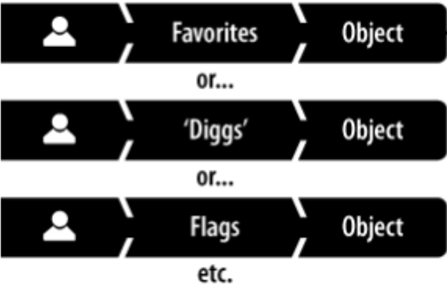
\includegraphics[width=5cm]{figures/rs_model_fav_and_flags.pdf} 
  \caption{Favorites, flags or send-to-friend models. (Source~\cite{farmer2010building})}
  \label{fig:rs_model_fav_and_flags}
\end{figure}

% TODO: Insert an image here

\subsubsection{Ratings}

Ratings model are used to get an explicit opinion about a reputable item. The upper and lower limit of the scale may vary from one variant to another. E.g. Internet Movie DataBase has a rating scale of 1 to 10, Google Play Store has a rating scale of 1 to 5. Ratings are gathered from multiple individual users and rolled up as a community average score for that target.

\begin{figure}[!htb]
  \centering
  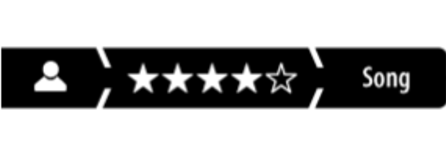
\includegraphics[width=5cm]{figures/rs_model_ratings.pdf} 
  \caption{Ratings model to rate individual objects. (Source~\cite{farmer2010building})}
  \label{fig:rs_model_ratings}
\end{figure}

\subsubsection{Reviews}

A review is a collection of ratings on different facets for a repuatble item. It also contains a text based freeform opinion.

\begin{figure}[!htb]
  \centering
  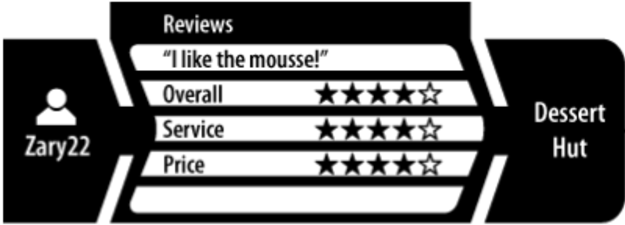
\includegraphics[width=6cm]{figures/rs_model_reviews.pdf} 
  \caption{Ratings include a text freeform opinion combined with other reputation models. (Source~\cite{farmer2010building})}
  \label{fig:rs_model_reviews}
\end{figure}

\subsubsection{Points}

Points are awarded to users based on their activity on the platform. If points are awarded properly, it encourages people to engage more on the platform, e.g. Stackoverflow awards users with points and badges for correctly answering questions. Please enage more for reputation.

\begin{figure}[!htb]
  \centering
  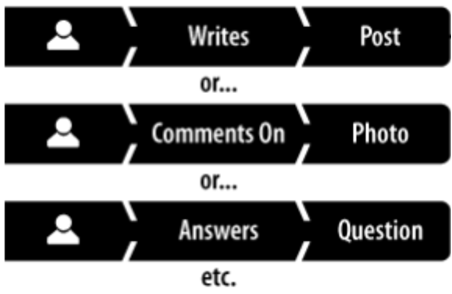
\includegraphics[width=5cm]{figures/rs_model_points.pdf} 
  \caption{Points are similar to favorites and flags but depends upon indirect action. (Source~\cite{farmer2010building})}
  \label{fig:rs_model_points}
\end{figure}

\subsection*{In context of S2Store}

\emph{Favorite and Flags} can be used as following:
\begin{enumerate}
  \item User can \emph{favorite or flag} an existing service.
  \item Developer can follow another developer.
  \item Developer can mark a context model as favorite, adding to its reputation.
\end{enumerate}

\emph{Ratings} can be combined with \emph{Reviews} to allow collection of qualitative feedback where users can express their satisfaction or frown with meaningful explanations.

\emph{Points} can be used in following ways:

\begin{enumerate}
  \item A point can be added to the service for each download. Uninstall would do the opposite.
  \item A point can be added to the context model for every service that associates itself with the context model.
\end{enumerate}

\subsection{Implicit Rating}
\label{subsec:implicit_rating}

In explicit rating, users explicitly tell the system what they think about something. Explicit rating gives accurate observation about an item. But explicit rating requires users to interrupt their normal browsing behavior \cite{claypool2001inferring}. Implicit rating uses less intruding methods. In general for e.g., users tend to read more articles than they rate. Users are also likely to review applications only if they find them very good or very bad \cite{Podkopajev2012}. Implicit rating evaluates the reputation through certain interest indicators based on user behaviors.

Girardello and Michahelles developed an app for Android called \emph{AppAware} as part of a voluntary research experiment \cite{girardello2010explicit}. The app collects events triggered every time a user installs, updates or removes any other app in their cell phones. These events are then shared with a central remote server. AppAware calculates the reputation of each app based on an assumption that good applications are not removed once installed, applications not liked are usually removed from the device. AppAware introduces an acceptance rate (reputation score) $v$ for an application $app$ as the value going from 0 to 100 computed with the formula in eq \ref{eq:appaware_a}, where $U$ is the set of users having at least one event for $app$ \cite{girardello2010explicit}.

\begin{equation}\label{eq:appaware_a}
  v(app)=\frac{\sum_{user \in U} last(app, user)}{|U|}
\end{equation}

\begin{equation}\label{eq:appaware_b}
  last(app,user) = \begin{cases}
    0 & \text{if last event for user for app = removed} \\
    90 & \text{if last event for user for app = installed} \\
    100 & \text{if last event for user for app = updated}
  \end{cases}
\end{equation}

According to eq \ref{eq:appaware_b}, the acceptance rate is based on the most recent event. \emph{Update} event is given more weight than \emph{install} because the assumption is that the user finds value in the app and keep it installed. \emph{Remove} event sets the acceptance rate to 0.

\subsection*{In context of S2Store}

The AppAware experiment from \cite{girardello2010explicit} shows good corelation between explicit rankings taken from Google's PlayStore and the collected implicit rankings. Therefore, eq \ref{eq:appaware_a} and \ref{eq:appaware_b} can be also used in S2Store. S2Store can track with the permission of user, when a new service is installed, uninstalled or updated and infer an implicit rating that can be combined with explicit rating to generate an aggregate reputation for services.
\section{App store simulation: AppEco}
\label{sec:analysis_appeco}

An ecosystem has a lot of moving parts and dynamic relationship between the actors inside the ecosystem \cite{Jansen}. One of the ways of studying such relationships is through simulation \cite{castiglione2006agent}.

Lim and Bentley did a comparative analysis of success of different strategies for developers while developing apps for a mobile app store \cite{lim2012successful}. They created a simulation of mobile app store ecosystems called AppEco. In AppEco, developer agents build and upload apps to the app store; user agents browse the store and download the apps \cite{lim2012successful}. They calibrate AppEco with suitable parameters that resembles the Apple's App Store and investigate the result by evaluating different developer strategies in terms of downloads received, app diversity and adoption rate.

We further explain the features of AppEco from \cite{lim2012successful} in the following section because they are relevant for our own simulation discussed in Chapter~\ref{chap:design}.

\subsection{AppEco Components}

In AppEco there are three components: apps, developers and users. In a real app ecosystem these three components form complex relationships, filling niches, competing and cooperating similar to a biological ecosystem \cite{lin2009operating}. In AppEco, apps, developers and users are abstracted models of their real world counterpart. Developer and user models are artificial life agents with certain behaviors. They are described below:

\subsubsection*{Developers}
\label{subsubsec:appeco_components_developers}

A developer agent takes $devDuration$ days to build an app and then uploads it to the app store. Developer keeps track of all of the apps she has developed. She uses one of the following strategies to build apps:

\begin{itemize}
  \item \emph{S0 Innovator} builds an app with random features each time.
  \item \emph{S1 Milker} try to milk an idea repeatedly. She makes an app and copies it with slight variations to produce many different apps.
  \item \emph{S2 Optimizer} makes variations in own best app each time. The strategy models developers who learn from their downloads and want to improve.
  \item \emph{S3 Copycat} copies app from the Top App Chart. The strategy models less creative developers but who want to achieve many downloads quickly.
  \item \emph{S* Flexible} begins with a strategy S0-S3. Each developer than has a 0.99 probability to pick an app from the Top App Chart list and to change the strategy to be the same as the developer of the selected app.
\end{itemize}

\subsubsection*{Apps}
\label{subsubsec:apps}

An App is developed and uploaded by the developer to the app store. Lim and Bentley show a novel way to model the different natures of an app by using a 10x10 feature grid.

\begin{figure}[!htb]
  \centering
  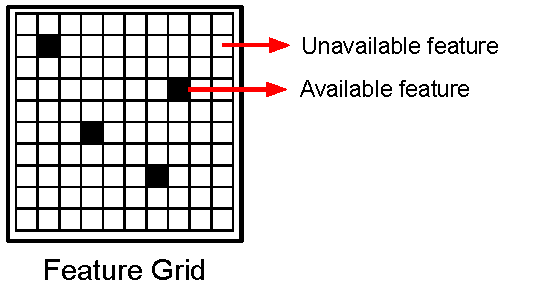
\includegraphics[width=9cm]{figures/example_service_grid.pdf}
  \caption{A grid representing an App. Black cells represent features and white cells represents lack of features. The coordinate of a cell represents its uniqueness.}
  \label{fig:example-grid}
\end{figure}

As shown in Figure~\ref{fig:example-grid}, a 10x10 grid can have white and black cells. A white cell is an empty cell and a black cell is filled cell. Each cell represents a unique feature identified by its x and y coordinates. In the figure, 4 of 100 cells filled, meaning the grid contains 4 out of 100 possible features. 

How each cell of the grid is filled depends upon the strategy of the app developer. We explain them below:

\begin{itemize}
  \item \emph{S0:} Each cell in the grid of the app is filled probabilistically. The probability of a cell being filled is given by $P_{Feat}$, one of the parameters for simulation calibration.
  \item \emph{S1:} For the first app, S1 also fills the cells as done by S0. For any further app, S1 copies the existing features of her first app and introduces random mutation. Mutation is explained below.
  \item \emph{S2:} For the first app, S2 also fills the cells as done by S0. Then the new apps are developed by copying features from her most successful (popular) app and introducing random mutation to it.
  \item \emph{S3:} One of the apps is randomly selected from the Top Apps Chart and its features are copied with random mutation.
\end{itemize}

The probability that a developer will mutate an app when copying is 0.5. During mutation, a developer picks one of the filled cells and moves its location to an empty cell.

\begin{figure}[!htb]
  \centering
  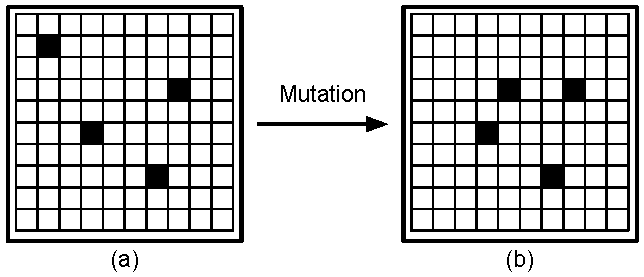
\includegraphics[width=9cm]{figures/example_app_grid_mutation.pdf}
  \caption{Example of grid mutation: One of the cells is randomly picked from (a) and moved to another location in (b).}
  \label{fig:example-grid-mutation}
\end{figure}

\subsubsection*{Users}

A user agent in AppEco downloads apps uploaded in the app store. The behavior of a user in AppEco is modeled as following:

\begin{itemize}
  \item Each user has a preference of what features she likes in her apps. The preference is also modeled using a grid (preference grid) as shown in Figure~\ref{fig:example-grid}. User agents use different probability $P_{Pref}$.
  \item Each filled cell in a preference grid represents a feature the user desires.
  \item If all the filled cells of the app grid are also filled in the preference grid of a user, the user downloads the app.
  \item A user keeps track of all the downloaded apps.
  \item A user takes a break of certain days before browsing the app store again for new apps. The number of days $daysBtwBrowse$ for each user is randomly selected between $[bro_{min}, bro_{max}]$ whose values are selected as part of simulation calibration.
\end{itemize}

\subsection{Algorithm}

The AppEco algorithm is responsible for modeling the interaction between the AppEco components mentioned in the section above. Each timestep in the algorithm represents a single day.

The population of developer and user agents grow following a sigmoid curve. The sigmoid curve follows the population growth as described in ecological studies given by Eq.~\ref{eqn:appeco_population_growth} \cite{lim2012successful}.

\begin{equation}\label{eqn:appeco_population_growth}
  pop_t=MinPop+\frac{MaxPop-MinPop}{1+e^{S*t-D}}
\end{equation}

Where, 
$pop_t  =$ the size of the population,
$MinPop =$ the minimum population,
$MaxPop =$ the maximum population,
$S =$ constant that determines the slope of the growth curve,
$D =$ constant that shifts the curve from left to right.


\begin{figure}[!htb]
  \centering
  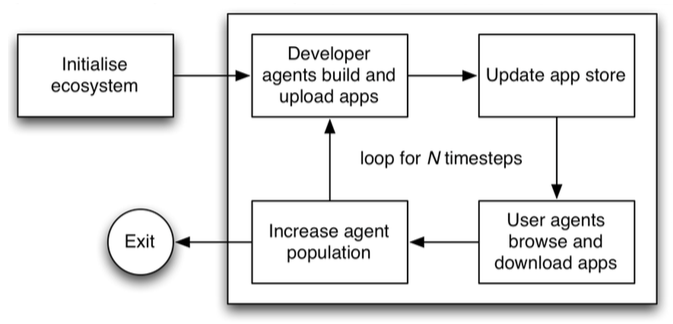
\includegraphics[width=11cm]{figures/appeco_algorithm.png}
  \caption{AppEco algorithm (Source:~\cite{lim2012successful}).}
  \label{fig:appeco-algorithm}
\end{figure}

The algorithm of AppEco is shown in Figure~\ref{fig:appeco-algorithm}. These steps are briefly described in the following section:

\subsubsection*{Initialize ecosystem}

The first step of AppEco is to initialize the system with timestep $t=0$. Most app stores have some apps before they launch to public. AppEco creates an initial number of app artefacts. AppEco also contains a pool of initial developers with all the strategies S0, S1 and S2 (S3 cannot start at $t=0$ because the Top Apps Chart is not ready yet). The initial app artefacts are assigned randomly to the initial pool of developers.

\subsubsection*{Developer agents build and upload apps}

For each day, active developers (subset of all developers) are selected based their $devDuration$. Each active developer uploads an app to the app store. Each developer then becomes inactive for the next $devDuration$ number of days before uploading another app. Developers can also become inactive based on probability $P_{Inactive}$.

\subsection*{Update app store}

In AppEco, the app store contains two charts:

\begin{enumerate}
  \item \emph{New Apps Chart} which includes the newest apps uploaded by users.
  \item \emph{Top Apps Chart} which includes the best ranked apps among all apps.
\end{enumerate}

For \emph{New Apps Chart}, any newly uploaded app has a probability $P_{OnNewChart}$ chance of appearing on it. There are maximum $N_{MaxNewChart}$ number of apps in the chart. Both variables are part of simulation calibration.

For \emph{Top Apps Chart}, the formula given by Eq.~\ref{eqn:appeco_app_ranking} is used to calculate the ranking of each app.

\begin{equation}\label{eqn:appeco_app_ranking}
rank = 8*D_1 + 5*D_2 + 5*D_3 + 3*D_4
\end{equation}

Where, $D_n$ is the number of downloads received by an app on the $n$th day before current day.
Like \emph{New Apps Chart}, there is a limit to the number of apps listed in \emph{Top Apps Chart} given by $N_{MaxTopChart}$.

\subsection*{User agents browse and download apps}

For each day, active users (subset of all users) are selected based on their $daysBtwBrowse$. Each of the active users browses the \emph{New Apps Chart} and \emph{Top Apps Chart} for the current day and downloads apps that match her preference grid. 

Users are also likely to search for a particular app based on their own requirements. Search however is simulated such that a random list of apps are shown to the user. The user then uses the same method as with the two charts described previously and downloads according to her preference. 

After download, each user waits for another $daysBtwBrowse$ number of days before becoming active and downloading another set of apps.

\subsection*{Increase agent population}

To simulate the growth of the ecosystem, the number of users and developers are increased for the next timestep using Eq.~\ref{eqn:appeco_population_growth}.

Each new developer is assigned $devDuration$ and each new user is assigned $daysBtwBrowse$ as explained previously.

\subsection{Simulation Results}

AppEco was calibrated using values for probability variables and other constants such that the growth of users, developers, apps and downloads matched the trend of the Apple's App Store. The total simulation was run for 1080 timesteps (3 years, 1080 days on average with 30 days per month). 

They give the following results:

\textbf{C1} According to AppEco, they found out that Copycat strategy S3 was the most successful with highest average downloads, top 20 downloads and top 20 average downloads \cite{lim2012successful}. Lim and Bentley back up the claim by giving example that when the app \emph{Angry Birds} was popular, the copycats had parasitised the app with clone of the app that successfully rose to the Top Apps Chart.

\textbf{C2} They claim that Innovator strategy produced the diverse apps fulfilling maximum users' preference for apps \cite{lim2012successful}.

\textbf{C3} They finally claim that S2 Optimizer strategy enables the developer to become more successful as they develop more apps although Copycat strategy is a winner in terms of number of downloads \cite{lim2012successful}. This is because copycats are plagiarising the work of other developers which eventually gets punished by the app store. The S2 Optimizer strategy produces an enhanced version of their apps which resembles the improvement developers make in real world by listening to user feedbacks.

Readers can refer to \cite{lim2012successful} for further interesting results from AppEco.

\subsection{Conclusion}

The AppEco simulation provides valuable insights to the nature of developers and users. Their results show which strategy are successful in terms of popularity, earnings and diversity. The also give valuable examples in real world that match their results.

The AppEco simulation is the first artificial life model of mobile application ecosystems \cite{lim2012successful}. The AppEco simulation presents a base example for doing further simulations on app stores.

The concept of grids is novel and can be applied to other entities where each entity can be compared to other entities in terms of similarities and differences. I.e., two grids having exactly the same number of filled cells in exactly same coordinates are equal and otherwise different. Grids also allow entities to undergo changes over time by mutation. Finally, grids allow to express complexity of entities based on the number of filled and unfilled cells.

AppEco uses a lot of random processes with different probability distributions during simulation. But with suitable calibration, it shows that through simulation, results can be achieve that mimic the results of a real life app store. This shows the suitability of the algorithm of AppEco.

In Section~\ref{sec:s2store_ecosystem} we describe the \emph{S2Store Ecosystem} which has elements similar to the one described here. In Section~\ref{sec:s2eco} we describe a simulation for S2Store Ecosystem based on AppEco.


\section{S2Store Ecosystem}
\label{sec:s2store_ecosystem}

The S2Store ecosystem like most ecosystems is expected to grow over time as the developers, their contributions and the number of users downloading them increase. The interaction becomes complex relationships, filling niches, competing and cooperating, similar to species in a biological ecosystem \cite{lim2012successful}. Ecosystem health is dependent upon community of developers that create innovative solutions that users want to use and the users providing relevant feedback back to the developers. The S2Store, central to the ecosystem allows anyone to build and publish their services. 

\begin{figure}[!htb]
  \centering
  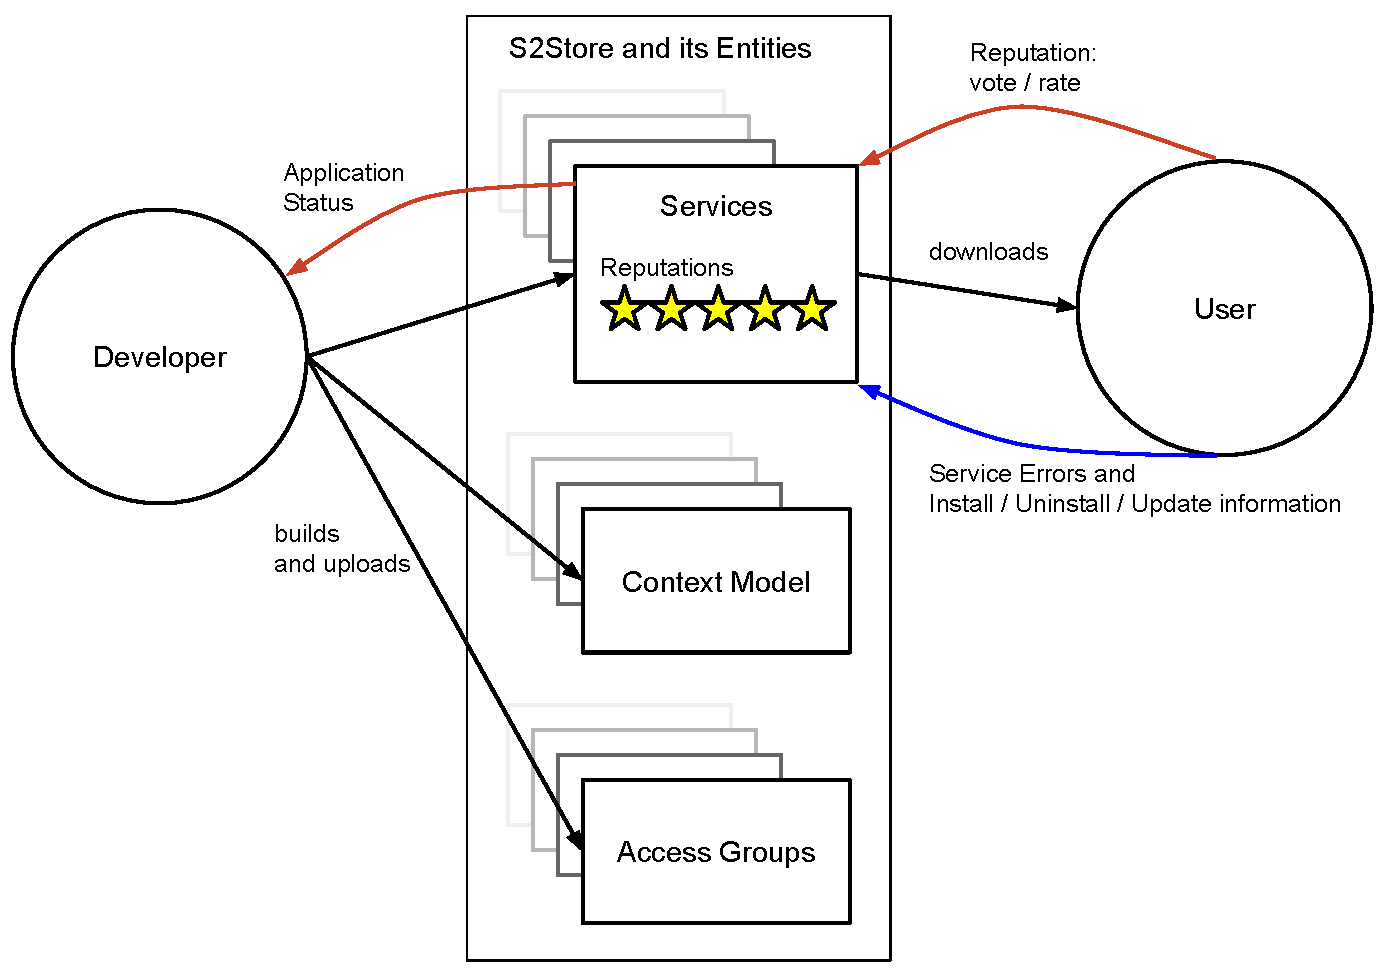
\includegraphics[width=15cm]{figures/ecosystem.pdf}
  \caption{Interaction between developers, entities and users in S2Store ecosystem.}
  \label{fig:ecosystem}
\end{figure}

\subsection*{S2Store Ecosystem Components}

S2Store ecosystem consists of developers, entities (context models, access groups and services) repositories and the users. Each component is described in detail below.

\subsection{Developers}

A developer is a registered user on the S2Store website who submits an application to the S2Store. Upon registration as a developer, she receies a \emph{developer-id} that is used to sign the application before submission. The developer-id is auto generated by the S2Store and unique per developer.

When creating a service for a smart space, a developer has to add the following entities:

\begin{itemize}
  \item Context-models that abstract the real world sensors or actuators or behaviors of desired smart space.
  \item Access-groups that group a set of resources and used to provide or revoke user permissions on these resources.
\end{itemize}

Context models and access groups are defined in Section \ref{subsubsec:context_model} and \ref{subsec:access_groups_and_convergence}. For both context models and access groups, a developer first searches if they exist already. When a suitable entity is found, a developer can reuse them in the service she develops. In case a suitable entity is not found, she can define new access groups and create new context models, submit to the S2Store and use them in her application.

The developer attaches a cryptographic signature to the application and submits it to S2Store. Once an application is marked as published, other users can download and install immediately.

A developer have access to multiple feedbacks collected by S2Store. She can see the statistics e.g. number of downloads, number of updates, removals, ratings by users. She can also see any comments and feedbacks submitted by users and respond back. S2Store can collect error logs submitted by applications and display them to developer so she can fix them.

A newer version of an application can be submitted to the S2Store. Users of old version are notified about the update.

\subsection{Context Model Repository}
\label{subsec:cmr}

Context Model Repository (CMR) deals with \emph{context models}. Context Models are briefly explained in the following section. We then explain their relationship with the CMR.

\subsubsection{Context Model}
\label{subsubsec:context_model}

A \emph{Context Model} is an abstraction of a context in a physical world into the virtual world. In VSL \si{\micro}-middleware, context models are expressed in XML.

\begin{lstlisting}[caption=A context model of a lamp., label=lst:lamp]
  <lamp>
    <isOn type="/derived/boolean">0</isOn>
    <dimLevel type="/basic/number" lowerBound="1" upperBound="5">3</dimLevel>
  </lamp>
\end{lstlisting}

The listing above is a context model of a real world lamp. It stores two attributes of a real world lamp: \texttt{isOn} and \texttt{dimLevel}. The default value for \texttt{isOn} is 0 - which relates to the lamp being turned off. The default value of \texttt{dimLevel} is 3 - which relates to the brightness level being in the middle of 1 and 5.

The VSL \si{\micro}-middleware reads these xml-templates of the context models and instantiates them with the default values. Services with either \emph{read} or \emph{write} permissions can perform respective activities on the context model instances. Permission and Security are explained in \ref{subsec:access_groups_and_convergence}.

\subsubsection{Context Model Hierarchy}

In VSL, context models form a hierarchical tree structure. The leaf nodes in the tree consist of three basic types provided by the system: number, string and list. The leaf nodes are \emph{inherited} to create complex sub-types. Advanced context models are created by \emph{composition} of simpler context models. In listing: \ref{lst:lamp}, a \texttt{lamp} definition is composed from another context models: \texttt{isOn} and \texttt{dimLevel}.

The following listing shows how a sub-type can be derived from the basic type.

\begin{lstlisting}[caption=Type inheritence: Sub type boolean is derived from /basic/number.]
  <boolean type="/basic/number" lowerBound="0" upperBound="1">
    0
  </boolean>
\end{lstlisting}

\subsubsection{Context Model Repository and Convergence}

The hierarchical tree structure of context models provides an additional benefit. Given a large number of developers involved in context modeling, we expect there would be a lot of duplicated effort. For e.g. multiple \emph{lamps} context models can exist from different developers or \emph{lamp1} could be of lesser quality than \emph{lamp2}.

The Context Model Repository is a central repository where developers can upload any context models they create. Each context model contains a globally unique identifier (guid). E.g. John can upload his context model at \texttt{/john/lamp1} and Jane can upload her context model at \texttt{/jane/lamp2}.

Other developers who want to program services for lamps can search for context model definitions of lamps. They see both John's and Jane's context models and decide on one of them.

With time, the number of context models increase in the CMR. Since context models link to each other, it forms a network that can be modeled with a directed graph. We can now calculate the importance of a context model in the global CMR space by analysing the number of forward associations and backward associations one context model has from its neighbours. The calculation of rankings of context models is explained in \ref{subsec:implicit_rating}.

Only developers interact directly with CMR, not the users. Developers can perform the following activities with the CMR:

\begin{description}
  \item[Validate:] A context model is dependent upon existing context models. CMR checks if the new context model definition is valid or not. It checks if the XML format is correct, whether the attributes passed to sub-nodes are correct, etc.
  \item[Upload:] A valid context model can be uploaded to the CMR. During upload, a developer requires the following information: \emph{xml, guid, tag set, description} where,

\begin{description}
  \item[xml] is the context model data.
  \item[guid] is the globally unique identifier. The scheme for the guid is similar to path structure for unix files and folders e.g. /username/device/abc/xyz/contextmodelname. First part of the guide is always namespaced with the username of the developer.
  \item[tag set] is a set of tags appropriate for the context model chosen by the developer.
  \item[description] describes the context model by writing what it is for, how it behaves and how others can use it. The description is used during full text search in the system. The rankings of the context models are dependent upon combination of internal and external reputation Section~\ref{sec:reputation_systems}.
\end{description}

\end{description}

% What are they, what do they do in DS2OS?
% How are they written. How do they interlink with others?
% How are access groups defined inside
% How services use these context models
% The relationship between context models and the CMR.
% How are they uploaded, deleted, downloaded and updated?

\subsection{Access Groups and Convergence}
\label{subsec:access_groups_and_convergence}

Any node in a context model metadata (xml) can be associated with certain access privilege by their authors. The privileges associated for read permission are \emph{readerIDs} and those associated for write permissions are \emph{writerIDs}.

\begin{lstlisting}[caption=Listing of lamp context model with \texttt{readerId} and \texttt{writerId} permissions.]
<lamp reader="lamp_readers" writer="lamp_writers">
  <isOn type="/derived/isOn" reader="*">
</lamp>
\end{lstlisting}

In the above listing, \texttt{lamp} context model defines two accessIds: \texttt{lamp\_readers} for read access and \texttt{lamp\_writers} for write access. Similarly the child node \texttt{isOn} has \texttt{*} as reader Id which signifies that it is publicly readable.

When building a service, a developer has to write the list of \emph{accessIds} her service is dependent upon. It is used by VSL to provide access control by comparing accessIds from the \emph{service certificates} with the Ids stored in the metadata of each context node.

Each context model developer is free to choose any accessId (readerId or writerId) for the nodes in the context model. Also, a developer can see the accessId associated with existing context models and reuse them.

Before submitting a context model to the S2Store, a developer should upload any new \emph{accessIds} with a human understandable description. Only then can she upload the context model. Otherwise the context model submission is considered invalid.

The convergence mechanism described earlier for context models also applies for the access groups. When significant amount of context models are uploaded in the CMR, comparably significant amount of accessIds are collected with their descriptions. This information is easily available to read online for other developers.

Multiple accessIds could account for the same security context. E.g. \texttt{lamp1} could offer \texttt{lamp\_reader1} and \texttt{lamp2} could offer \texttt{lamp\_reader2}. However, the more a specific context model is used, the more its access group becomes popular.

Popularity calculation is done through a reputation system discussed in Section~\ref{sec:reputation_systems}. Popularity affects the ranking where an access group appears during search.

\subsection{Service Store and Convergence}

Services in the DS2OS are analogous to apps in the Apple AppStore or Google PlayStore. They are written in Java and utilize a fixed application programming interface (API) provided by DS2OS to interact with the VSL. DS2OS provides mechanisms for managing services within a Smart Space through Service-to-Space (S2S) Section~\ref{sec:ds2os}. Services can perform various different activities and are classified accordingly into following classes \cite{pahl2014distributed}:

\begin{enumerate}
  \item \textbf{Adaptation Services} connect Smart Devices to the VSL.
  \item \textbf{Advanced Reasoning Services} infer new context from existing VSL context.
  \item \textbf{Emulator Services} emulate the behavior of a service, e.g. an adaptation service that interfaces a Smart Device.
  \item \textbf{Remote Access Services} provide access to functionality in a remote DS2OS site.
  \item \textbf{User interface Services} provide a User Interface (UI) for DS2OS services.
  \item \textbf{Primary context providers} extend the semantics that can be used to identify context nodes.
\end{enumerate}

The different service classes reflect the wide variety of applications. The potential use cases for a service are vast.

Before a service is uploaded in the S2Store, the corresponding context model and access groups should also be uploaded. Then the service package is created that consists of the following contents:

\begin{itemize}
  \item \textbf{The service executable} An executable java package file in Java ARchive (JAR) format.
  \item \textbf{A service manifest file} contains basic information about the service e.g. unique service name, developer id, version number, cryptographic hash of the service executable, etc.
  \item \textbf{The service certificate} also contains some duplicate information as in the service manifest file but also contains additional fields like access groups (readerIDs and writerIDs) that it needs permission to, ModelId of the context model that belongs to the service, cryptographic hash of the context model and cryptographic hash of the manifest file.
\end{itemize}

The service package can now be finally uploaded to the S2Store.

\subsection{Users}

A user is someone interested in using the DS2OS to create smart spaces. Users download, configure and run the DS2OS their computing environments. DS2OS being a distributed system can run in multiple computing nodes. DS2OS provides an interface to interact with the packages in the S2Store. Users can perform the following activities:

\begin{itemize}
  \item \textbf{Browse} S2Store for top services or most recent services.
  \item \textbf{Search} S2Store for services according to users' preference and their available smart devices.
  \item \textbf{Install or Uninstall} a service and be able to run it or remove it.
  \item \textbf{Rate} a service according to the perceived quality.
  \item \textbf{Comment} about the service to send a public feedback.
\end{itemize}

\subsubsection{Browse}

Users can browse previously uploaded services in the S2Store by visiting the website. There are two lists that users can browse to discover new services.

\begin{itemize}
  \item \textbf{List 1: Recent Services} sorts the services by the date when they were uploaded. The recent uploaded services are displayed at the top.
  \item \textbf{List 2: Popular Services} sorts the services by the reputation ranking of the services. How reputation of a service is calculated is discussed in Section~\ref{sec:reputation_systems}.
\end{itemize}

In both lists, users are able to filter by the tags associated with the services. For e.g. a user can filter the listing to show services related with only \emph{lighting}.

\subsubsection{Search}

S2Store contains a search interface for users to browse existing apps. The interface is similar to those provided by existing mobile AppStores. E.g. Figure~\ref{fig:search-interface-play-store}

\begin{figure}[!htb]
  \centering
  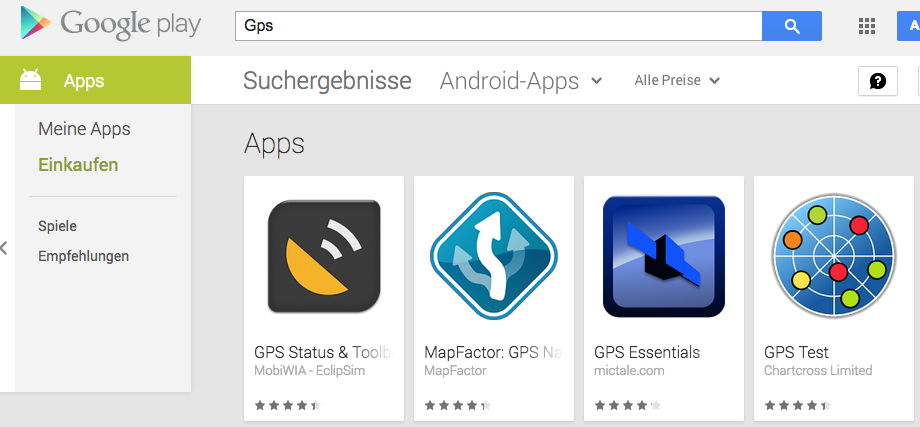
\includegraphics[width=14cm]{figures/search-interface-play-store.png}
  \caption{Search interface of Google's Play Store. (Source~https://play.google.com/store)}
  \label{fig:search-interface-play-store}
\end{figure}

% Search results are listed to the user according to a ranking algorithm discussed in \hl{TODO link to ranking algorithm discussion}

\subsubsection{Install or Uninstall}

DS2OS provides users with an interface to install a service into their local system. It will automatically download the software from the S2Store. Users can also keep track of available updates to existing services and uninstall them when necessary. Feedbacks are collected from these actions with the consent of the user. 

\subsubsection{Rate}

On the webpage of S2Store, users can rate any services they want. There exist different rating mechanisms discussed further in Section~\ref{sec:reputation_systems}. Ratings help to collect explicit feedback about a service from the users.

\subsubsection{Comment}

Comments are a common way to express user opinion on the internet. Comments serve multiple purposes in the S2Store. Users can comment to express satisfaction, dissatisfaction, request for new features in the service, report bugs, etc. Constructive comments help developers identify bugs and improve their services \cite{pagano2013user}.

\section*{Conclusion}

Reputation Systems in S2Store can bring convergence to hosted entities: services, context models and access groups. The Reputation Systems come in different varieties and one solution does not fit all. We analyzed and identified which models provides what kind of features and will look into how they suits S2Store.
\section{Research Questions and Methodology}
\label{sec:research_questions_and_methodology}

The following statements from \cite{pahl2014distributed} are of interest in the thesis:

\begin{enumerate}
  \item ``Having a statistic of the popularity of a model, it is likely that service developers in a crowdsourced development scenario orientate at the popularity as most popular context models are likely to be supported in most Smart Spaces in the world.''
  \item ``Collecting the error statistics and usage statistics can help providing users with feedback about the reliability and the use of a service which can be used to conclude about the quality and usefulness of a service.''
\end{enumerate}

We can now ask the following questions:

From \textbf{1}, 
\begin{itemize}
  \item[] \textbf{Q1} Is the assumption valid?
  \item[] \textbf{Q2} What happens if developers orientate or do not orientate towards the popularity of existing?
\end{itemize}

From \textbf{2},
\begin{itemize}
  \item[] \textbf{Q3} Is the assumption valid?
\end{itemize}

In both cases, we want to see how these statements can be validated. We are aware of two methodologies discussed below:

The modern scientific study of a phenomenon generally consists of three major approaches: theoretical, experimental and computational \cite{castiglione2006agent}.

\emph{Theoretical Study} for Smart Spaces have not been found. Most likely it is an dynamic and evolving at the moment.
% is not not so useful with AppStore study because AppStore is a moving and constantly changing structure with no formally defined precise behavior of humans: developers and users. Specially in an evolving field like smart spaces, theoretical study is unsuitable.

\emph{Experimental Studies (ES)} were done by \cite{pagano2013user} and \cite{chen2011predicting}. They make predictions based on the existing data by feeding them into different prediction models. 

\emph{Agent-based Modeling (ABM)} was used by \cite{lim2012successful} to simulate the behavior of users in App Ecosystem.

Both approaches have their advantages and drawbacks. Experimental studies are suited when existing facts based data are available.

In this thesis, we instead pick Agent-based Modeling because of the following reasons:

\begin{enumerate}
  \item The dynamics of entities association differs in S2Store compared to existing mobile app stores. So not having existing data suits ABM compared to ES \cite{castiglione2006agent}.
  \item ABM allows us to make variations in our assumptions and investigate the outcome \cite{castiglione2006agent}.
  \item ABM has been tested in economics, social sciences, ecology and many other fields which are relevant to ecosystem we are working with \cite{lim2012successful}.
\end{enumerate}
\chapter{Related Work}

Pahl presents \emph{Smart Space Store (S2Store)} which is an App Store for smart spaces. He argues that S2Store can be as revolutionary for smart space ecosystem as App Store was for Apple's ecosystem \cite{pahl2014distributed}.

An explanation of the dynamics inside an app store is presented in \cite{Jansen}. It lists the roles of individuals involved: users, developers, platform maintainers and how they interact with each other. It also compiles a list of required features and policies present in six existing Mobile app stores. It is interesting to see that Reputation Mechanisms like voting and app review are standard part of all of the mobile app stores. This is relevant to the thesis particularly because app stores interact with hundreds of thousands of developers \cite{lim2012successful} and reputation systems help to maintain an order in the system.

The benefits of Reputation Systems have been widely studied \cite{Akerlof1970} \cite{Axelrod1984} \cite{Resnick2000} \cite{farmer2010building}. The advantages and challenges in building Reputation Systems are presented in \cite{Resnick2000}. Different Reputation System models and their use case scenario are presented in \cite{farmer2010building}. The benefits of explicit rankings are well known but implicit rankings are not. Implicit rankings are a part of growing trend of measuring user behavior online to understand them better \cite{claypool2001inferring}. An example of effectiveness of implicit ranking algorithm is presented in \cite{girardello2010explicit}.

One of the major problems in building softwares for smart spaces in the diversity of smart devices. It is difficult to build a software for lamp that can work in majority of housing systems with different models of lamps. Cook et. al proposes a solution of all new smart devices to contain unique tags based on a consistent semantics \cite{Cook2012}. Pahl argues that building semantic ontology is a difficult proces given the existing variety devices at scale \cite{pahl2014distributed}. He proposes to use the dynamics of crowdsourcing this process. Existing studies prove empirically that a central software repository is very helpful for collaborative development irrespective of geographical position \cite{dabbish2012social}. Users are very likely to provide helpful feedback to developers through the app stores \cite{pagano2013user}. So, the crowdsourcing concept can be extended to collaboratively build an ontology of smart devices  based on popularity of their use \cite{pahl2014distributed}.

Simulation of an app store helps to observe the dynamic process inside the S2Store. Lim and Bentley \cite{lim2012successful} observed the correlation of using different strategies by developers to their success by simulating Apple's App Store. The simulation is called AppEco. It is an artificial agent-based model simulation that abstracts developers, users and apps in suitable models and adds them with behavioral assumptions. They have further used AppEco in different experiment to answer more questions. Thus AppEco has been used as a based model on top of which Smart Space Ecosystem (S2Eco) has been created as part of the thesis.

Entities involved in S2Eco: developers, users, software, context models, access groups have interconnections with each other. During simulation large number of entities are created. The structure of growth of graph has been studied in mathematics. When connections are chosen randomly, it creates a random graph. Random graphs do not depict the real nature of interconnection in software systems. According to LaBelle and Wallingford \cite{labelle2004inter} who studied the inter-package dependency networks in open source software, software system graphs have scale-free degree distributions, exhibit small-world effect and have assortative mixing \cite{newman2002assortative}. These properties have also been confirmed by simulations done in \cite{myers2003software}. It is desirable to have these properties in the simulation of S2Eco.

\chapter{Design}
\label{chap:design}

The focus of the thesis are the questions asked in Section~\ref{sec:research_questions_and_methodology}. We asked ourselves how we can verify convergence happens for context models, access groups and services with the S2Store. We looked into DS2OS (Section~\ref{sec:ds2os}) and how it provides portability (Section~\ref{sec:portability}). S2Store allows us to achieve portability through convergence (Section~\ref{sec:portability}). We analyzed app stores and their features (Section~\ref{sec:introduction_to_an_app_store}). We analyzed what reputation systems are, how they are put together and how they function (Section~\ref{sec:reputation_systems}). We analyzed how app stores can be studied with the help of simulation (Section~\ref{sec:analysis_appeco}). We finally analyzed the S2Store ecosystem and explained what convergence mechanism are and what benefits they provide (Section~\ref{sec:s2store_ecosystem}). 

In the following sections, we describe the elements we borrow from our analysis to answer our research questions.

\section{Modified AppEco for S2Store : Introduction}
\label{sec:s2eco}

An S2Store is also an app store because it shares the same features and requirements as found in the general definition presented by \cite{Jansen}. Like in a mobile app store, S2Store has users and developers. The difference is that while in a mobile app store, developers and users engage through apps, in S2Store they engage through services. Services are more complex compared to apps because of lack of standards and portability reasons (Section~\ref{sec:portability}). S2Store not just hosts one type of entity: services but also other entities like context models and access groups (Section~\ref{sec:s2store_ecosystem}).

AppEco simulation has provided with valuable insights in answering questions related to app stores. We extend AppEco for S2Store by introducing a similar simulation called \emph{S2Eco}. Through S2Eco, we observe the behavior of the smart space ecosystem and try to find the answers of our questions. Significant parts of the AppEco simulation has been explained in Section~\ref{sec:analysis_appeco}. With this as base, we expand the simulation to suit for S2Store. The additions and changes are explained in the following sections.

Like AppEco, S2Eco consists of artificial model agents. In addition to developer and user agents, S2Eco contains artifacts like services, context models and access groups instead of apps in AppEco. Developer agents develop services with corresponding context models and access groups and upload them to the S2Store. Users browse the S2Store and download the services. Users can then provide positive or negative feedback about the services online.

Each entity and its interactions are explained in the following section:

\section{Developer Agents}

The developer agent in S2Eco has all of the behavior of the developer agent in AppEco. But instead of building apps, they build services. Each developer agent requires \emph{devDuration} days to build a service such that: $$devDuration \in [dev_{min}, dev_{max}]$$

Each developer is initially active and continues to build and upload the services. However she has a chance to become inactive with a probability of $P_{inactive}$. This models hobbyist, part-time developers, and the tendency of developers to stop building services. Each developer uses one of the following strategies to build the services:

We could model a developer to alter between the four strategies described in AppEco (Section~\ref{subsubsec:appeco_components_developers}): S0 Innovator, S1 Milker, S2 Optimizer or S3 Copycat. There is however a significant difference here: mobile app stores are more competitive marketplace than cooperative and collaborative platform. In contrast; for S2Store, collaboration is a significant element (Section~\ref{sec:portability}). Specially for developers, we assume that developers behavior are more collaborative and less competitive \cite{dabbish2012social}. Hence in S2Eco, we only consider S0 Innovator and ignore the rest of the strategies.

Due to feedback mechanism available in app stores, developers are constantly notified with the feedbacks received from users. The way by which they react to the feedbacks are different. We create three different categories to place the developers based on their possible reactions to feedbacks: \emph{Improver}, \emph{Ignorer} and \emph{Malicious}.

\begin{itemize}
  \item \textbf{Improver} fixes all the bugs from the applications she owns. This models the individuals who improve their applications constantly.
  \item \textbf{Ignorer} do not care about the feedback. This models developers who submit their application once and chooses not to improve them regardless of feedback from users.
  \item \textbf{Malicious} developers are those who add additional bugs into their software. They model beginner developers who are not proficient with development. This also models developers who intentionally add malicious features to the apps once these apps get famous.
\end{itemize}

\emph{Hypothesis 1} Depending upon the category of a developer, the average rating of the services has distinct behavior per category. Services by \emph{Improvers} should have strong improvement on rankings over time and should cause higher downloads. Services by \emph{Ignorers} should show a constant or slightly decreasing average ratings over time. Services by \emph{Malicious} developers should show decrease in rankings over time.

\emph{Hypothesis 2} The ratings of context models and access groups would strongly correlate for \emph{Improvers} because popularity of services bring visibility to the associated context models and access groups. The chance that other developers also use the context models increase with increased visibility. However since context models are immutable, decrease in ranking of services due to \emph{Ignorers} and \emph{Malicious} developers should not affect the reputation of already uploaded context models.

\section{Services}

A service entity models an actual service uploaded in the real S2Store. It is modeled exactly similar to an app in AppEco. It is built and uploaded to the S2Store by developer agents. The features of a service are abstracted as a 10x10 feature grid $F_s$ for each service. Each cell in the 10x10 grid is a feature. If a cell is filled in $F_s$, then the service offers that particular feature.

The service feature grid $F_s$ is filled with a probability of $P_{featS}$ as shown in Figure: \ref{fig:example-service-grid}.

\begin{figure}[!htb]
  \centering
  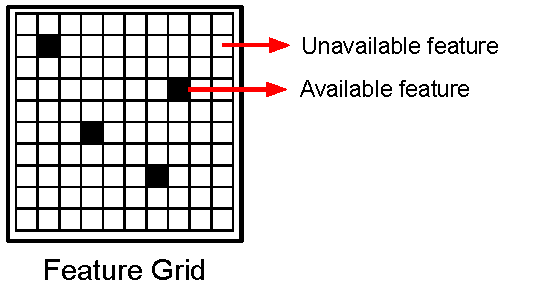
\includegraphics[width=9cm]{figures/example_service_grid.pdf}
  \caption{Example of a service grid. Each cell is filled with a probability of $P_{featS}=0.04$. A cell filled with black at row=r and col=c represents that it has a feature at coordinate r,c}
  \label{fig:example-service-grid}
\end{figure}

Various types of services have been discussed in Section~\ref{subsec:access_groups_and_convergence}. For artificial life simulation, we remove the differences between them and generalize all services to behave in one simple way: their features are randomly generated.

A service entity stores the day when it was created to identify if it is a new service or not. 

In S2Eco, service entities have two major roles.

\begin{enumerate}
  \item They store reputation scores calculated by S2Store. These scores change over time. The change in score is measured and analyzed (Section~\ref{sec:experiments}).
  \item Service entities dictate the popularity of context models by virtue of their inter-relationship. The more service entities use a context model, the popular it becomes in comparison to other context models. We also observe this behavior in S2Eco (Section~\ref{sec:experiments}).
\end{enumerate}

\section{Devices}
\label{sec:devices}

A device entity models the presence of wide variety of devices in the market. A device model represents the abstract concept of the utility of the device. For example, A washing machine is an abstract concept with predefined set of utilities (should be able to wash clothes, should have a connector to water supply, etc). But we can find different designs, brands and models of washing machines in the market. Here, the device entity would model the concept of a washing machine.

Devices entities are associated with Context Model entities discussed below. Ideally for portability reasons, each device would have one context model. But crowd sourced development means different developers come up with their own designs that fit their purpose. A device entity can be associated with many different services.

\section{Context Models}
\label{sec:context_models}

Context models have been explained in Section~\ref{subsec:cmr}. They abstract the context in a physical world into the virtual world. When a developer designs a service, the service uses the context models to communicate with different devices and other services. So a service is always associated with at least one context model, if not many.

A developer writes down the list of context models her service uses before packaging the service and uploading it to the S2Store. Context model entities in S2Store save the relationship between context models and services. In each timestep of the simulation, the number of relationships between services and devices are counted to give a popularity ranking to the context models. The more a context model is associated with different services, the more popular it is.

Whenever a developer thinks about creating a service, she starts with the problem. She then identifies the solution and the list of devices she can use to build the solution service. She goes on to the S2Store and checks the CMR for a list of context models suitable for the device. The S2Store will show her all similar context models that suit her device along with the reputation score of each context model.

It does not always have to be a device for a developer to search a context model. Context models can represent other abstract concepts, act as a common data store, etc independent of any association with physical devices. However, for simplicity reasons, we assume all context models are derived from devices.

Thus, all context models in S2Eco are also associated with devices. By default, a context model is always associated with one device in the simulation while this is not necessary in real world. This has been done again to simplify the simulation.

Context models are also associated with other context models as they form hierarchical structures. Simple context models that represents simple devices are combined together to describe a complex context model that represents a complicated device. For e.g., a context model for an automated window will depend upon context models for automated hinges, open and close switch for window blinds, ambient light and wind sensors etc. Second, a developer has to specify in any service she develops, which context models the service is dependent upon. For e.g., an automated window control service will specify context models for a temperature sensor and on/off switch control. These two context models have an internal connection in the system.

We also assume that context models evolve over time. At the beginning when the platform has not gained wide spread adoption with developers, context models are simpler: have less features. With time, context models with higher complexity are created.

The features in a context model are also abstracted as a 10x10 feature grid $F_{cm}$ as with apps in AppEco (Section~\ref{subsubsec:apps}). Each cell of a $F_{cm}$ is filled with a probability of $P_{featCM}$. In contrast to the fixed probability value $P_{Feat}$ for apps in AppEco or the probability value of $P_{featS}$ of the services, the probability of a context model $P_{featCM}$ is a linear function of timesteps. As time progresses, $P_{featCM}$ increases as shown in Eq.~\ref{eqn:linear_context_model_function}.

\begin{equation}\label{eqn:linear_context_model_function}
P_{featCM}(t) = P_{featCMmin} + \frac{P_{featCMmax} - P_{featCMmin}}{T_{total}} * t
\end{equation}

Where, $T_{total}$ is the current timesteps or total number of days for simulation.

\begin{figure}[!htb]
  \centering
  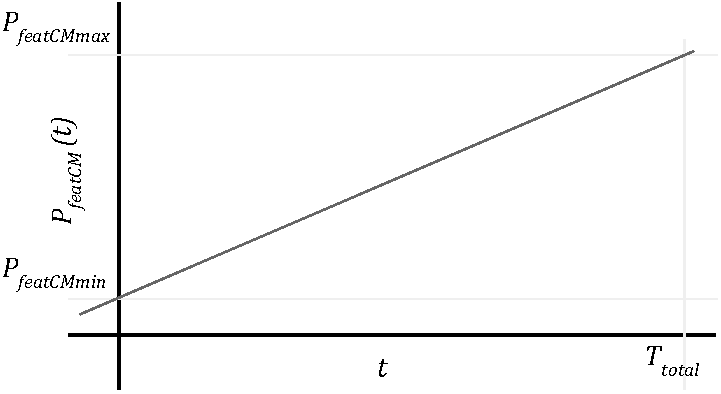
\includegraphics[width=12cm]{figures/probability-of-feature-vs-time.pdf}
  \caption{Linear relationship between $P_{featCM}(t)$ and time $t$.}
  \label{fig:probability-of-feature-vs-time}
\end{figure}

\begin{figure}[!htb]
  \centering
  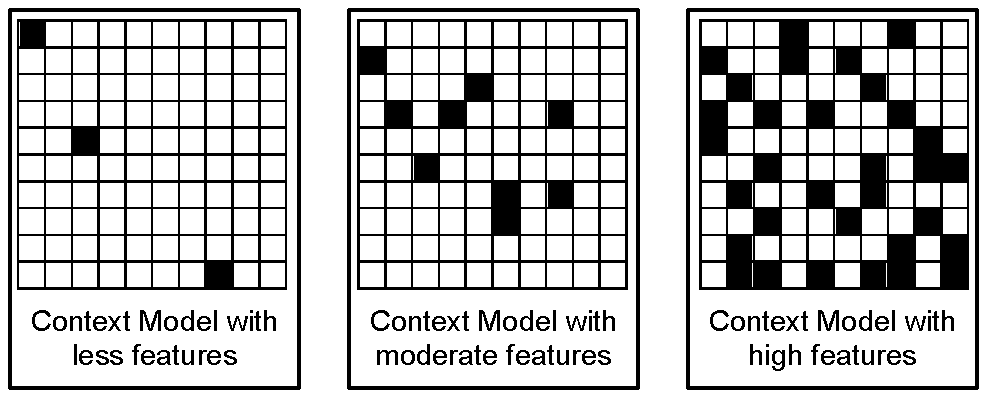
\includegraphics[width=12cm]{figures/feature-level-of-context-models.pdf}
  \caption{Amount of features of context models increase with time.}
  \label{fig:feature-level-of-context-models}
\end{figure}

Linear growth of $P_{featCM}(t)$ with time $t$ can be seen in Figure~\ref{fig:probability-of-feature-vs-time}. It results in context models getting more complicated over time as shown in Figure~\ref{fig:feature-level-of-context-models}. There are three context models with increasing number of filled black cells from left to right. The context model on the left is the least complex and the one on the right is the most complex in terms of number of features.

We assume that simpler context models have less dependencies with other context models while complex context models have higher dependencies with other context models.

To illustrate this, we take an example of two context models. A simple automatic lamp can depend upon \emph{an ambient light sensor}, \emph{a switch}, \emph{own light source}. A complex room automation system depends upon a lot of context models of higher abstractions like \emph{lighting}, \emph{temperature control}, \emph{music and multimedia control}, \emph{personal assistance} etc which themselves are complex and depend upon lower abstractions.

We model this behavior such that a context model with $x$ features depends upon $N$ other context models where $N$ is given by,

Given $\textbf{Y}$ is a random independent variable,
\begin{equation}
  \begin{aligned}
    Y &\in [0, 1],\\
    N &= Y * f(x),\\
    f(x) &= N_{min} + \frac{N_{max} - N_{min}}{100} * x
  \end{aligned}
\end{equation}

\begin{figure}[!htb]
  \centering
  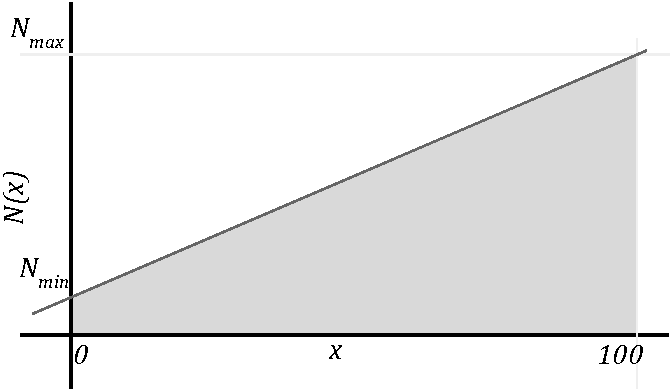
\includegraphics[width=12cm]{figures/num-of-context-models-vs-features.pdf}
  \caption{The gray portion represents the number of context models $N(x)$ associated with a new context model with $x$ number of features. A complex context model with large features has probability to have higher number of related context models.}
  \label{fig:num-of-context-models-vs-features}
\end{figure}

\begin{figure}[!htb]
  \centering
  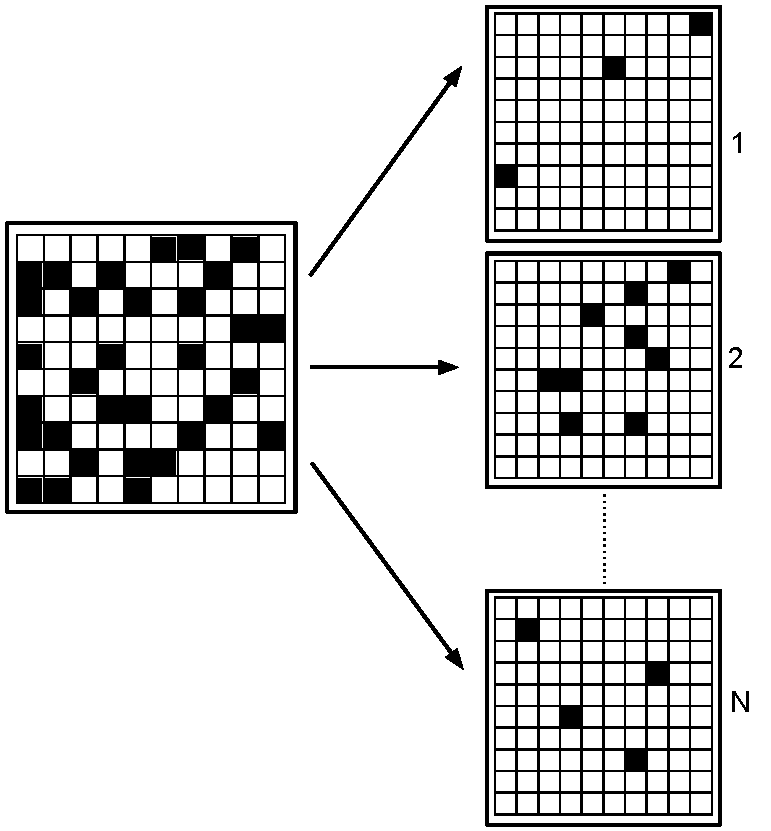
\includegraphics[width=8cm]{figures/context-model-dependency.pdf}
  \caption{A context model dependent upon N other context models.}
  \label{fig:context-model-dependency}
\end{figure}

The increase in context dependencies from one context to another is shown in Figure~\ref{fig:num-of-context-models-vs-features}. Figure~\ref{fig:context-model-dependency} shows a context model on the left dependent upon $N$ other context models on the right.

By modeling increase in complexity of context models and the increase in dependency of a context model to other context models, we assume that S2Eco is slowly evolving over time. We used the linear growth as suits better than other models because it gives more predictable result during simulation.

\subsection{Ranking of Context Model}

In real world S2Store, developers search for these dependent context models. They have a particular feature requirement and search for other context models that provide these features. Developers can search by category or by text. The search results are ordered according to the ranking of each context model.

\begin{figure}[!htb]
  \centering
  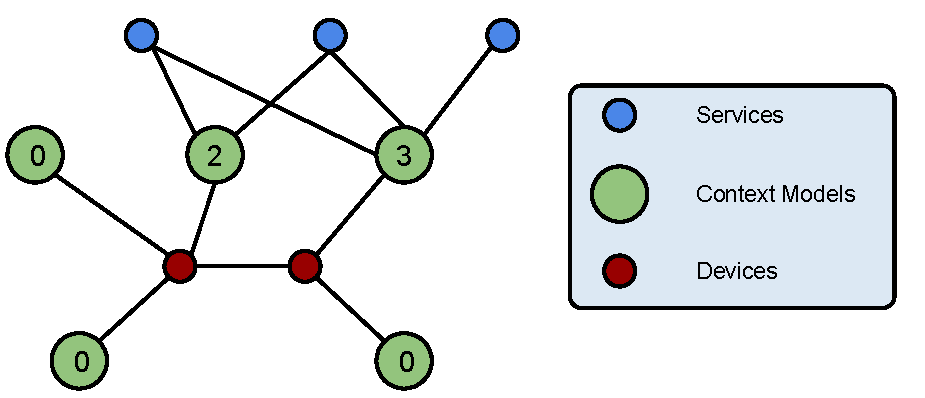
\includegraphics[width=10cm]{figures/association_between_context_models.pdf}
  \caption{Association between context models through services. The numbers inside the context models show the \emph{Reputation Value}.}
  \label{fig:association-between-context-models}
\end{figure}

Ranking of a node determines its popularity. Associations between context models can be modeled in a graph where each context model is a node and the association with other context models is represented as a edge as shown in Figure \ref{fig:association-between-context-models}. Popularity of a context model is calculated as a centrality measure. Different centrality measures exist. In S2Eco, we use the number of services that use a context model as its reputation score. For e.g., if 15 services mention context model $c$, then $R(c)=15$ where $R$ is a reputation function.

\subsection{Algorithm of how a developer chooses a context model}

An active developer when creating a new service, decides on the devices she wants to associate in the service. The number of devices for a service is chosen randomly between [1, $D_n$] where $D_n$ is a function dependent upon the simulation timesteps. As timesteps increase, a developer is likely to choose more devices for her services.

This is based on the expectation that at the beginning of the ecosystem, most of the services contributed are likely to be adaptation services that allow future services to take advantage of real world devices. In future, the number of devices associated per service increases.

She then searches the S2Store for existing context models matching the devices. She is either satisfied and chooses the existing context model or she is unsatisfied and decides to create her own new context model.

A device ends up having multiple context models. When a developer searches for existing context model, we want her to be able to find the one which is used the most by other developers. This behavior is simulated such that the probability of a developer choosing a particular context model depends upon how many existing services already use it. The probability distribution is given by $$P_{selectCM}(x)=\left\vert{E(x,y)}\right\vert$$ where $E(x,y)$ is a set of all associations of the context model $x$ with any existing services. A context model is five times more likely to be picked by a developer if it is already used by five existing services than another context model that is used by only one existing service.

\section{User Agents}

Each user agent has preferences that determine the service features that it prefers, similar to user preference in AppEco. The preferences of a user agent are also abstracted as a 10x10 preferences grid ($\textbf{U}$). The cells in $\textbf{U}$ are filled probabilistically, such that each cell in the grid has a probability of $P_{Pref}$ of being filled. If a cell in $\textbf{U}$ is filled, then the user agent desires the feature represented by that cell. If the feature grid of a service $F_s$ has a cell in the same location filled, then it means the service offers a feature desired by the user agent. In Figure \ref{fig:user-service-feature-matching}, all four of the features offered by Service 1 match the user agent's preferences, but only two of the features offered by Service 2 match the user agent's preferences. The matching is binary, so either the cells match or do not match.

\begin{figure}[!htb]
  \centering
  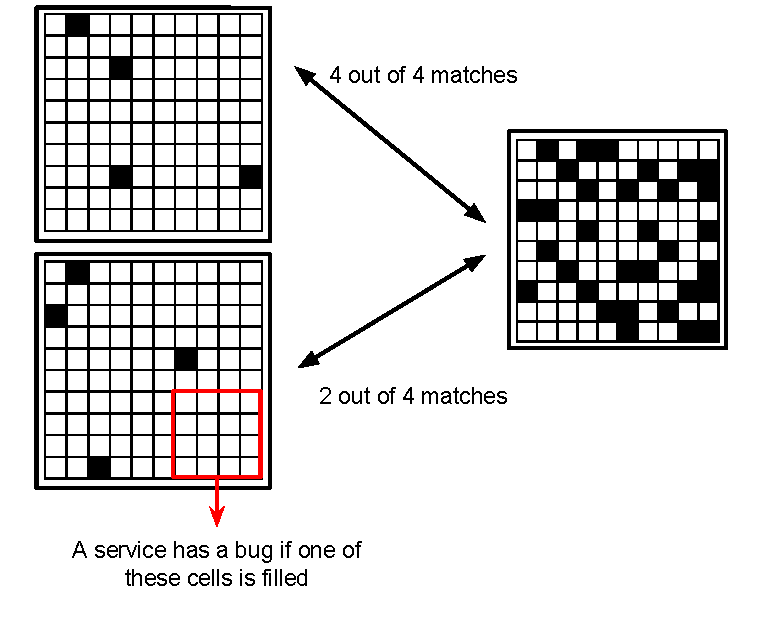
\includegraphics[width=10cm]{figures/user_service_feature_matching.pdf}
  \caption{Matching service features with user preferences}
  \label{fig:user-service-feature-matching}
\end{figure}

A user agent keeps record of the number of services it has downloaded and the number of days between each browse of the S2Store ($daysBtwBrowse$, a random value between $[bro_{min}, bro_{max}]$), and the number of days that have elapsed since it last browsed the S2Store ($daysElapsed$). $daysElapsed$ is recorded so that the user agent knows when to browse the app store next. When a user is initialized, the $daysElapsed$ is set to a random number between $[0, daysBtwBrowse]$ so users don't all browse at the same time when they start.

\section{S2Store}

S2Store is used by the agents to store and access \emph{Context Models} and \emph{Services}. For developers, it allows to see access groups and context models uploaded by other developers. Developers can search for a context model based on number of features as explained in \ref{sec:context_models}.

Users can use the S2Store to browse the services. There are three methods for browsing: Top Services Chart, New Services Chart, Keyword Search. Top Services Chart lists the services based on their reputation. New Services Chart lists the services based on the date of upload (latest services appear at the top). Keyword search is abstracted as random search for random service.

\section{Algorithm}

Our algorithm based on the AppEco algorithm from \cite{lim2012successful}. It models the interaction between the components described in previous sections. Each timestep in the algorithm represents a day in the real ecosystem.

Population growth of the developers and users is modeled using a sigmoid growth function commonly used to model the population growth in natural systems. The equation models the growth rate of users and developer agents in an app ecosystem declining as their population density increases. The population size at timestep $t$, $pop(t)$ is defined by 

\begin{equation}\label{eq:s2eco_algorithm}
  pop(t)=MinPop + \frac{MaxPop - MinPop}{1+e^{S*t-D}}
\end{equation}

where $MinPop$ is the minimum population, $MaxPop$ is the maximum population, $S$ determines the slope of the growth curve and $D$ shifts the curve from left to right.

The algorithm is shown in Figure \ref{fig:algorithm-flow} and explained below:

\begin{figure}[!htb]
  \centering
  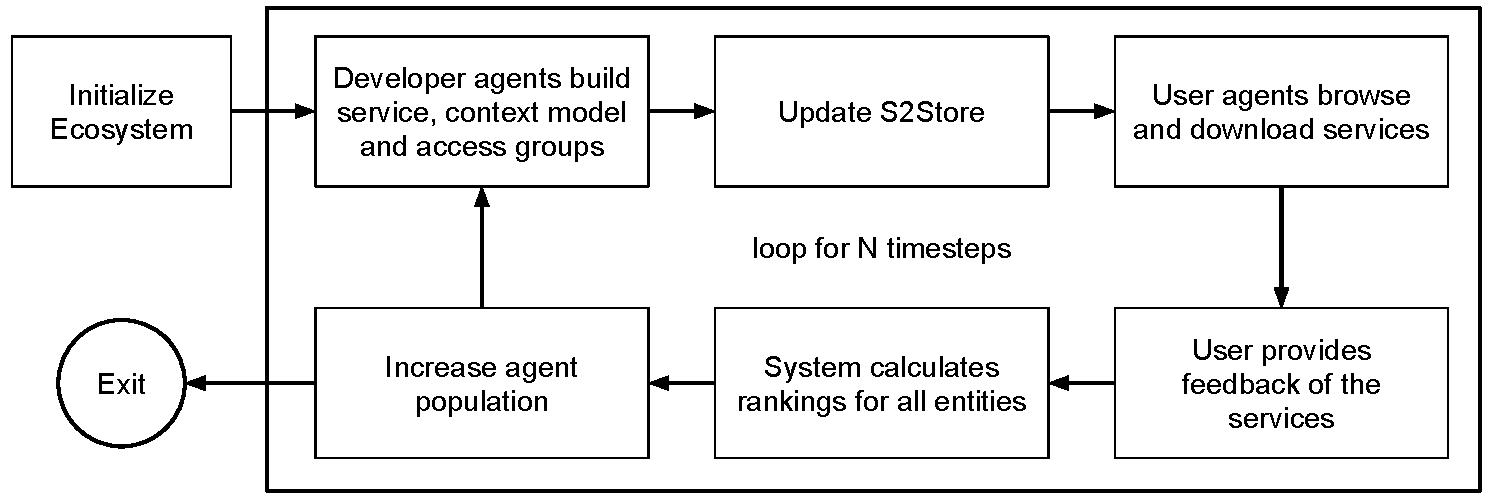
\includegraphics[width=13cm]{figures/algorithm-flow.pdf}
  \caption{Matching service features with user preferences}
  \label{fig:algorithm-flow}
\end{figure}

\subsection{Initialize ecosystem}

The step launches S2Eco with the population of developer and user agents as defined in \ref{eq:s2eco_algorithm}, with timestep = 0.

\subsection{Developer agents build services, context models}

For each active developer, \emph{daysTaken} is incremented by 1. If \emph{daysTaken} exceeds the developer's \emph{devDuration}, the development of service is completed. Developer then uploads the service to the store, resets \emph{daysTaken} to 0, and decides on the next service to build. The feature grid $F$ of the service is set as described earlier.

Any new context models created when creating the service are also uploaded to the S2Store.

The developer also goes through her old services to see if they have bugs as reported from the users. The developer then acts according to his nature. \emph{Innovator} removes the bugs, \emph{Ignorer} ignores the bugs while \emph{Malicious} user introduces new bugs. The modified services are then uploaded to the S2Store.

\subsection{Update S2Store}

New Services Chart contains $T_{newServices}$ number of latest uploaded services ordered by the latest service on top. Top Service Chart list is also updated so that services are ranked in the order of decreasing score, calculated as $8*D_1+5*D_2+5*D_3+3*D4$ where $D_N$ is the number of downloads received by the service on the \emph{n}th day before the current day.

\subsection{User agents browse and download services}
For each user, \emph{daysElapsed} is incremented by 1. If \emph{daysElapsed} exceeds \emph{daysBtwBrowse}, then the user browses the S2Store, and resets \emph{daysElapsed} to 0. User browses New Services Chart and the Top Services Chart as well as conducts Keyword Search. Keyword Search returns a random number of services from the S2Store. User filters through all the services by matching her preference grid with the feature grid of the services. For e.g., in Fig \ref{fig:user-service-feature-matching}, the user downloads Service 1 but not Service 2.

\subsection{User agents provide feedback of the services}

In this step, all users who browsed the S2Store goes through their newly downloaded services. If a service has a bug, the user votes randomly between 1 and 2. If a service has no bug, the user votes randomly between 3,4 and 5.

\subsection{System calculates rankings for all entities}

This step calculates and stores the average rating of all the services.

\subsection{Increase agent population}

This step increases the number of devices, users and the developers in S2Eco for the next time step, using Eq. 1.

\section{Discussion}

We now have a structure for the S2Eco simulation. It contains all the basic necessary elements that interact with one another: developers, users, services, context models and access groups. There are limitations to the simulation because in real life, the behaviors are very complex. We have not attempted to capture many of these complexities. We have a basic system with the smallest amount of features that allow us to answer our questions.

The simulation focuses on the quality of services delivered by the users and the kind of user feedbacks provided back into the system. This should show us interesting patterns in terms of increased ratings and increased number of downloads. The simulation also focuses in popularity of context models depending upon the number of services that use a particular context model or inter context model relationships. By altering the nature of how these inter-relationships occur, we can see how the relationships evolve and how soon a context model becomes popular among other similar competing context models.
\chapter{Evaluation}

In order to investigate the dynamic behavior of the simulation, we must first calibrate the system by choosing our parameters. Most parameters have been inspired by the AppEco experiment which itself uses Apple's App Store chronological data for the calibration.

\section{Calibration}

The parameters used for simulation are shown in Section~\ref{list:simulation_params}. The growth of developers, users, services and devices are shown in Figure~\ref{fig:growth_dev_user_services}.

\begin{figure}[!htb]
  \centering
  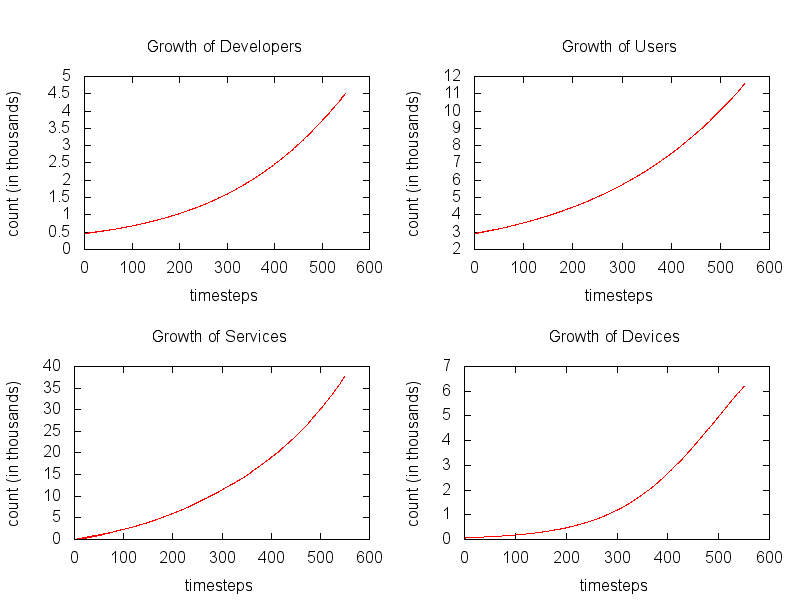
\includegraphics[width=14cm]{figures/dev_user_service_device.png}
  \caption{Growth of developers, users, services and devices over time}
  \label{fig:growth_dev_user_services}
\end{figure}

Growth of population for users and developers are a part of sigmoid growth as explained in Eq.~\ref{eq:s2eco_algorithm}. The growth of services increases exponentially over time. This is because as the population increases, the number of active developers per day increases producing more services. The growth of developers also follow a sigmoid curve but with different parameters. The assumption is at the start of the simulation, developers are interested in less number of devices. As time increases, the variety of devices that developers are interested also increase.

We run the simulation for around 550 timesteps (550 days).

\section{Implementation}

The simulation was coded in Ruby and the graphs were drawn using Gnuplot. Ruby is not as fast as C and C++ but was chosen due to author's familiarity with the language. The simulation takes significant amount of processing time (one day to simulate 100,000 developers and 400,000 users). The simulation is thus broken down into two parts:

\begin{itemize}
  \item User vote simulation. This simulation is focused on observing feedback of users on services.
  \item Context model convergence simulation: This simulation is focused on how context models are reused by developers and how they form their network.
\end{itemize}

\section{Experiments}
\label{sec:experiments}

\subsection{User vote simulation for service convergence}

\textbf{Q} How does user feedback affect the services?

To answer the question, we ran the simulation for 550 timesteps (equivalent to 550 days). For each category of developers: \emph{Improvers}, \emph{Ignorers} and \emph{Malicious}; we observed the average rating of the services uploaded to the S2Store. The following graph as shown in Figure~\ref{fig:votes_distribution_segregated} was observed.

\begin{figure}[!htb]
  \centering
  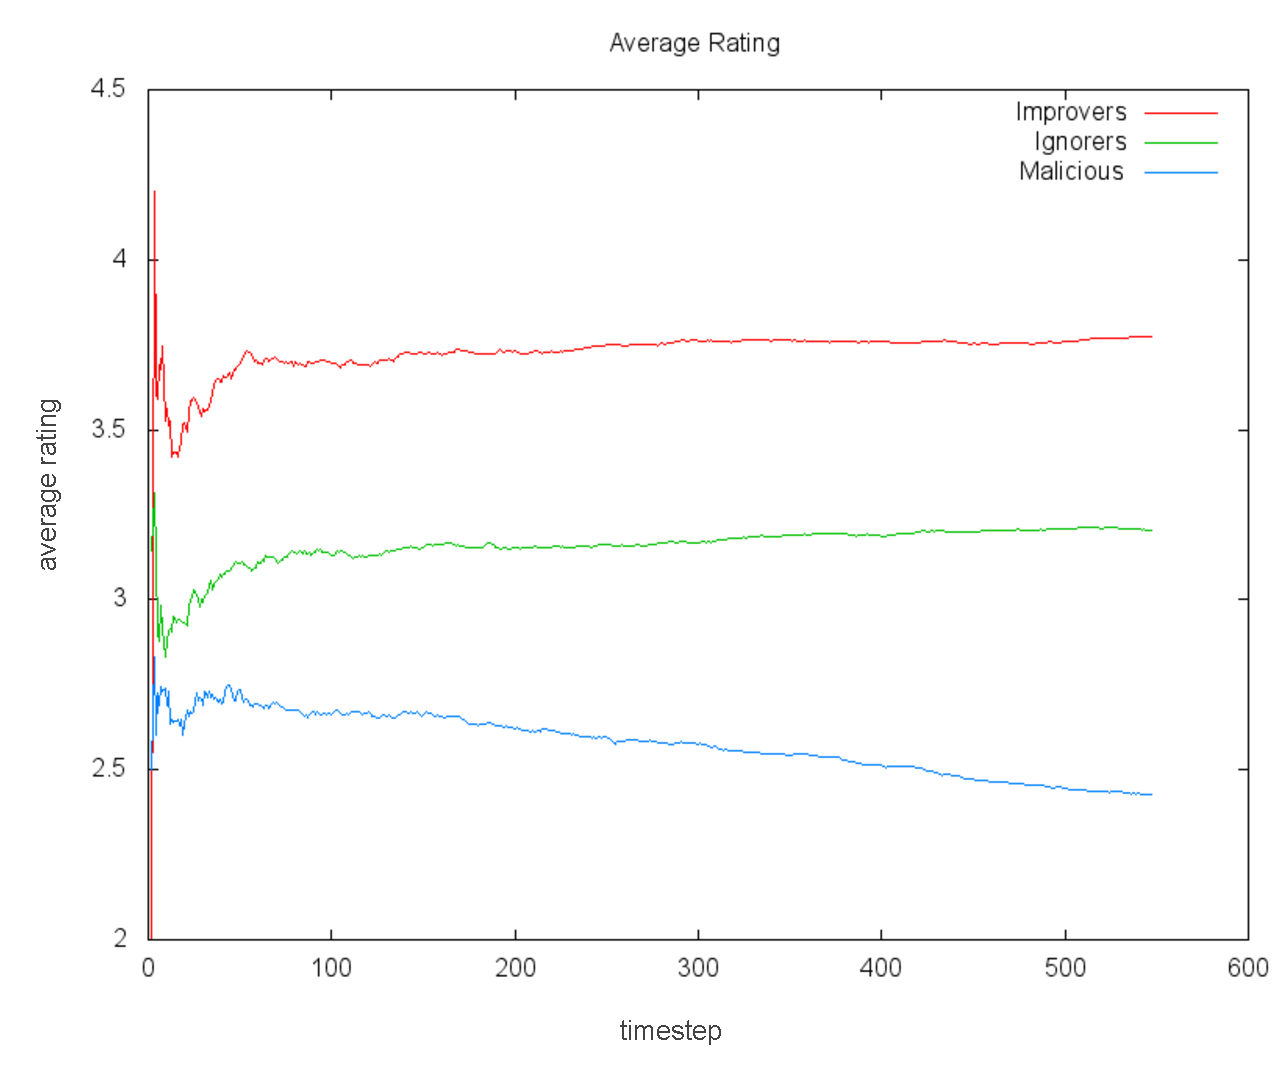
\includegraphics[width=13.5cm]{figures/votes_distribution_segregated.pdf}
  \caption{Distribution of votes among among Improvers, Ignorers and Malicious Developers}
  \label{fig:votes_distribution_segregated}
\end{figure}

Figure~\ref{fig:votes_distribution_segregated}, shows the average vote received under each category of developers. The red line shows the average vote for \emph{Improvers}, the green line shows the average vote for \emph{Ignorers} and the blue line shows the average vote for \emph{Malicious} developers.

The average vote for \emph{Improvers} stay around 3.75 out of 5 and increases gradually. While the average vote of \emph{Ignorers} also stay around 3.2 out of 5, the ratings for \emph{Malicious} users decrease gradually over time.

From this Figure~\ref{fig:votes_distribution_segregated}, we can interpret that a developer who is constantly improving the quality of her app is liked by the users more. Users are happy to see bugs fixed in the applications they use. 

Surprisingly for \emph{Ignorers} the average rating did not decrease as expected. We believe the reason for this behavior is that in S2Eco, all services are equally likely to receive votes between 1 and 5. Since \emph{Ignorers} choose not to change anything, the average rating stays around 3.

Unsurprisingly for \emph{Malicious} developers, users quickly discover the presence of bugs of malicious contents and rate them either 1 or 2. Hence the overall average rating of the services fall down gradually.

\begin{figure}[!htb]
  \centering
  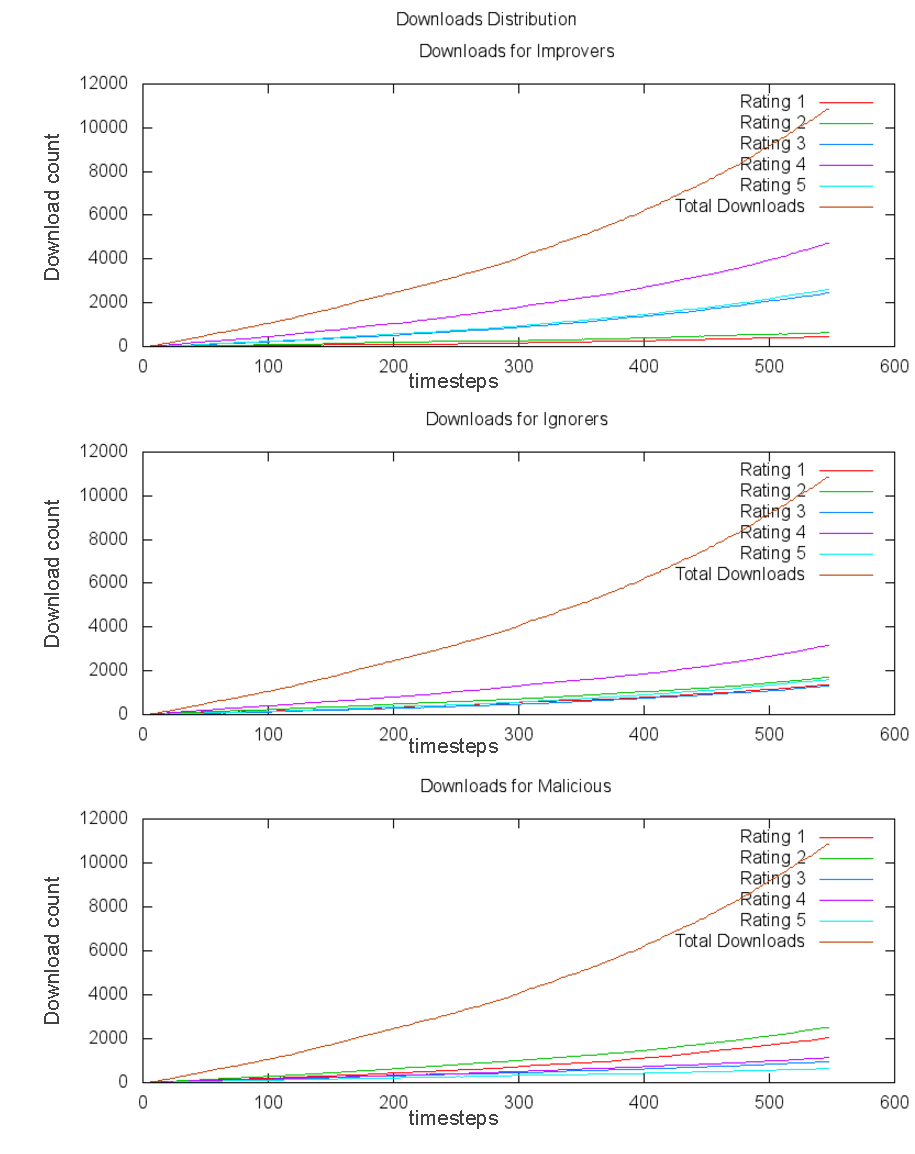
\includegraphics[width=13.5cm]{figures/plot_downloads_segregated.pdf}
  \caption{Distribution of votes among among Improvers, Ignorers and Malicious Developers}
  \label{fig:plot_downloads_segregated}
\end{figure}

From the graph in Figure: \ref{fig:plot_downloads_segregated}, we see that the total number of downloads received by services developed by all three categories remain the same. This is shown by the red top most line in all three graphs. The reason why different categories did not receive different download counts was because in current simulation, users decision to download a service is not influenced by existing rating of that service. User only provides a feedback into the system once she has downloaded and installed the service.

Since \emph{Improvers} constantly improve their services, in long term the users using these services have better experience compared to other categories. This is seen from the first graph where for \emph{Improvers}, most downloaded services have an average rating of 4 while services with 1 and 2 ratings are least downloaded. In contrast in second and third graphs, services with any ratings are equally downloaded.

\subsection{Developer and device interaction simulation for context model convergence}

\textbf{Q} How does developer behave with different information from S2Store and how it affect context model convergence?

To answer the question, we look at the graph shown in Figure: \ref{fig:result_component_relationship}. The three connected cliques are related to three devices (red circle). Each of the devices are connected with three, one and two context models (green) and each of these context models are connected with services (blue circle).

\begin{figure}[!htb]
  \centering
  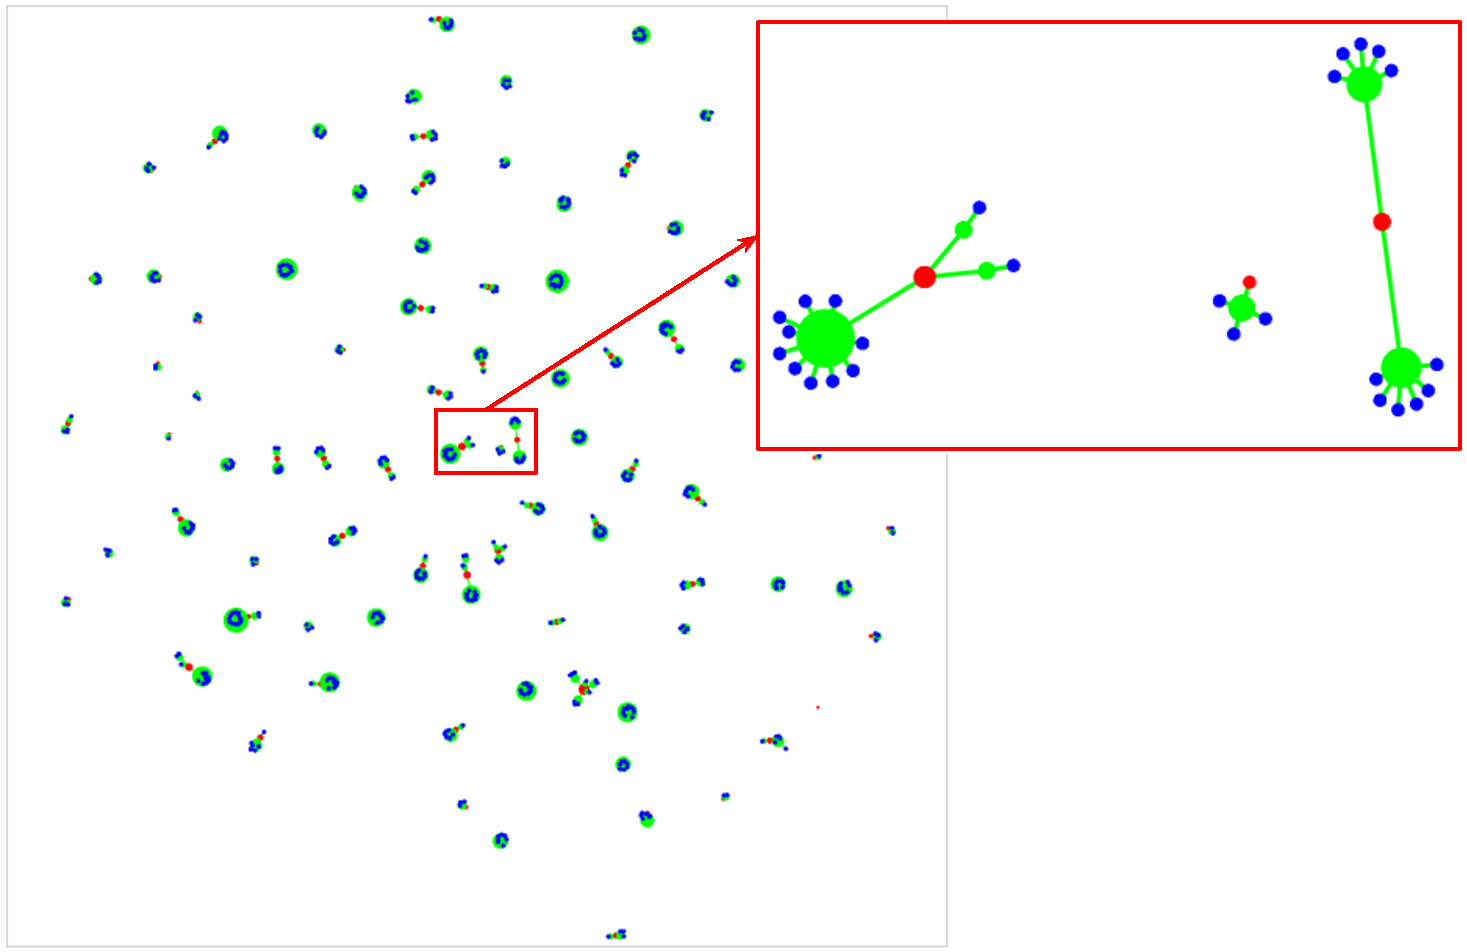
\includegraphics[width=13cm]{figures/result_component_relationship.pdf}
  \caption{Inter-relationship between devices (red), context models (green) and services (blue) at timestep = 25 days}
  \label{fig:result_component_relationship}
\end{figure}

At the beginning of the simulation, S2Eco only produces services that are likely to have only one context model and thus only one device. However, different services can refer to the same device, with different context models. In the figure, the size of the context models (green circle) shows the number of attached services to it.

\begin{figure}[!htb]
  \centering
  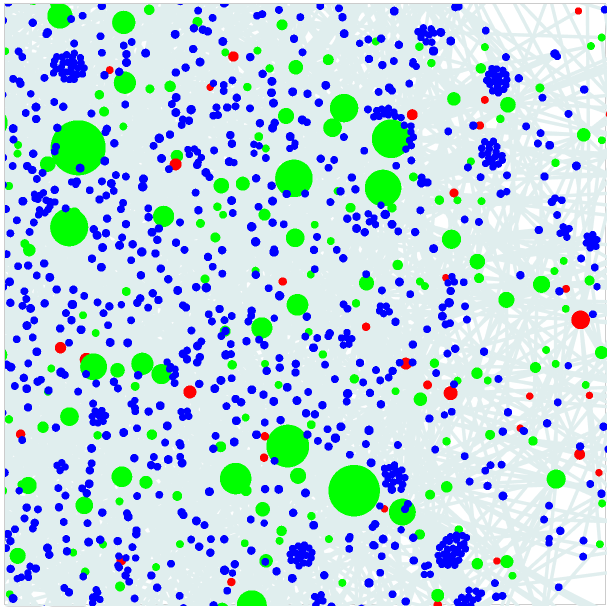
\includegraphics[width=9cm]{figures/result_component_relationship_99.png}
  \caption{Inter-relationship between devices (red), context models (green) and services (blue) at timestep = 99 days}
  \label{fig:result_component_relationship_99}
\end{figure}

After 99 timesteps, the graph was seen as in Figure: \ref{fig:result_component_relationship_99}. The edges have been removed to make the image more clear. It can be seen that more popular context models (larger green circles) have more services (blue circle) around its periphery. Smaller context models have less services around their periphery. The trend increases as the simulation progresses.

\begin{figure}[!htb]
  \centering
  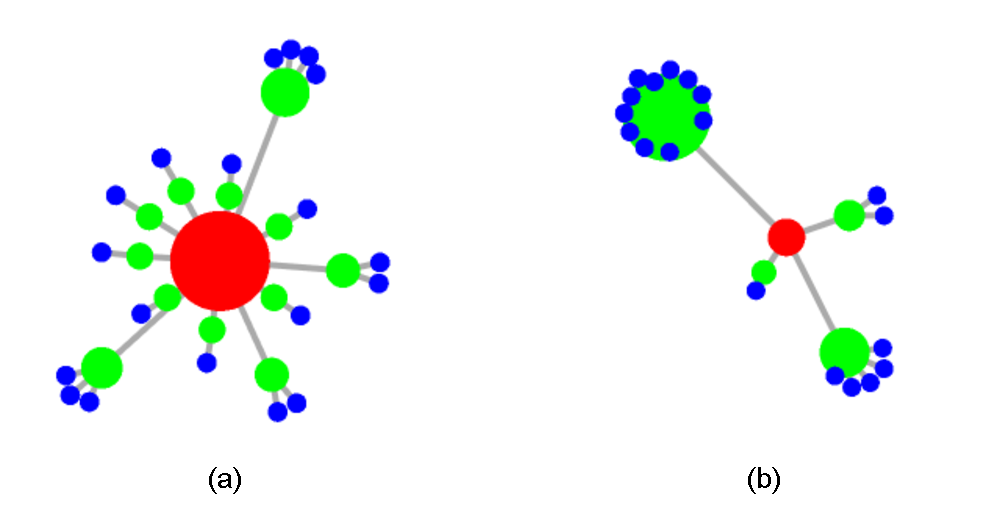
\includegraphics[width=9cm]{figures/result_compare_graph_user_personality.pdf}
  \caption{Two graphs resulting from two different experiments. Graph on the left (a) has a device at the center (red) with many context models associated with it. The context models are almost equal is their degree centrality. There is no clear favorite here. Graph on the right (b) has less context model and one context model is a clear favorite with many services attached to it.}
  \label{fig:result_compare_graph_user_personality}
\end{figure}

It is important for S2Store to be able to provide information about existing context models and their statistics to the developers. A developer is more likely to reuse existing context model when she finds the detail she is looking for. To see how this affects the production of context models, we simulate it in S2Eco. There are two different experiments associated with the graphs in Figure: \ref{fig:result_compare_graph_user_personality}. In the first experiment, developers  had less information. So they had equal probability to either choose existing context model or create a new one themselves. In the second experiment, developers had more information. So the chance that they would select existing context model to creating a new one was $10:1$.

In the first experiment, developers contribute duplicate context models to the store. There are more context models per device with each service using its own context model. Thus, they are not portable with each other.

In the second experiment, there are less context models per device. One context model is a clear favorite among the developers as they contribute more services to it than other context models. The group of services that are dependent on the same context model are compatible and take benefit from each other.

\chapter{Conclusion and Future Work}
\label{chap:conclusion_and_future_work}

\section*{Conclusion}

In this thesis, we observed how convergence occurs for context models and services in a smart space ecosystem. We argued that significant challenges in encompassing smart devices in smart spaces can be solved by the architecture presented in DS2OS with Smart Space Store (S2Store). We created a simulation S2Eco which involves the necessary elements in a real life smart space ecosystem based on Distributed Smart Space Orchestration System (DS2OS). During simulation, developer and user agents were programmed to have different behaviors. Various parameters influenced how the S2Store presented developers with different list of latest, top services and search results. We used the voting mechanism to simulate user feedbacks.

The assumptions made during the simulation were very simplified. Developer characteristics were not scientifically assigned but based on emperical reasoning. The relationships and complexity of context models were also based on reasoning rather than a scientific comparison. The algorithm used to calculate rankings was a very simple algorithm based on downloads. A different choice of ranking algorithm should show significant changes in the convergence process. A real world implementation of the algorithm should combine different features like download counts, manual user voting, implicit rating based on user actions, etc which were lacking in our implementation.

However, we observed that the presence of S2Store as a central point of collaboration between developers and users causes the quality of software services to grow. We also saw when developers are aware of existing popular context models contributed by other developers and reuse them, convergence occurs for context models.


\section*{Future Work}

The simulation has some limitations which we list below and suggest further development ideas for them:

\begin{itemize}
  \item User behavior simulation: In the simulation we have assumed developers to always be \emph{Innovators} during service production. More developer types like \emph{Copy Cats}, \emph{Optimizers} and \emph{Milkers} can be added.
  \item During service creation, it selects the devices randomly from existing pool of devices. This algorithm causes the network of device, context models and services to form a random graph. It can be optimized by selecting devices that are already inside a closer circle. In real life, this means that a service is more likely to use different devices that have been used together before.
  \item \emph{Top services list} algorithm considers only the downloads in the last four days. The algorithm can be improved by making a user aware of rankings provided by other users.
\end{itemize}


The Speed of simulation was slow. It took the simulation around 30 minutes to run for 600 timesteps and it increases exponentially as timesteps are increased. This included simulating service creation, upload, top lists generation, user preference matching, voting etc for above 12,000 users and 5,000 developers. To improve the simulation, we recommend the architecture be modified to take advantage of concurrency and also rewrite to C or C++.

\appendix{}
\newgeometry{top=1cm,bottom=0.1cm}

\chapter{Simulation Parameters}

\begin{equation}\label{list:simulation_params}
  \begin{aligned}
    DAYS\_TOTAL &= 550 \\
    P\_FEAT\_CM\_MAX &= 100 \\
    P\_FEAT\_CM\_MIN &= 1 \\
    P\_FEAT\_S      &= 0.04 \\
    P\_PREF\_USER   &= 0.45 \\
    NUM\_CM\_MAX &= 70 \\
    NUM\_CM\_MIN &= 1 \\
    DEV\_MIN, DEV\_MAX &= [1, 90] \\
    P\_INACTIVE &= 0.0027 \\
    POP\_MAX\_DEV &= 20000 \\
    POP\_MIN\_DEV &= 100 \\
    S\_DEV       &= -0.005 \\
    D\_DEV       &= -4.0 \\
    POP\_MAX\_USER &= 80000 \\
    POP\_MIN\_USER &= 1500 \\
    S\_USER       &= -0.0038 \\
    D\_USER       &= -4.0 \\
    BROWSE\_RANGE &= [1,360] \\
    KEY\_WRD\_MAX  &= 200 \\
    U\_AVOID\_SIZE &= 3 \\
    BUGGY\_SIDE     &= [6,9] \\
    P\_VOTER        &= 0.2 \\
    P\_APPS\_TO\_VOTE &= 0.5 \\
    TOP\_NEW\_SERVICES  &= 50 \\
    TOP\_BEST\_SERVICES &= 50 \\
    POP\_MIN\_DEVICES &= 5 \\
    POP\_MAX\_DEVICES &= 10000 \\
    S\_DEVICES       &= -0.01 \\
    D\_DEVICES       &= -5.0 \\
    P\_SERVICE\_DEVICE\_MIN &= 1 \\
    P\_SERVICE\_DEVICE\_MAX &= 50
  \end{aligned}
\end{equation}

\restoregeometry

 % TODO: remove if glossary not needed
% \glsaddall{} % add all defined terms to glossary, even if not referenced in text
% \printglossaries{}

\microtypesetup{protrusion=false}
\listoffigures{}
% \listoftables{}
\microtypesetup{protrusion=true}
\printbibliography{}

\end{document}
